\documentclass[11pt, a4paper]{article}
\usepackage[utf8]{inputenc}
\usepackage[spanish]{babel}
\usepackage{amsmath, amssymb, amsfonts}
\usepackage{graphicx}
\usepackage{geometry}
\geometry{left=2.5cm, right=2.5cm, top=2.5cm, bottom=2.5cm}
\usepackage{tikz}
\usepackage{bm}
\usepackage[hidelinks]{hyperref}
\graphicspath{{figs/}{../figs/}}


\title{\vspace{-1.5cm}\textbf{Resolución de Ecuaciones Diferenciales Ordinarias}\\ \large Métodos Matemáticos I --- Hoja 4}
\author{\textbf{César Endris Acosta}}

\date{22 de octubre de 2026}
\begin{document}

\maketitle
\vspace{-0.2cm}

\begin{center}
\fbox{\parbox{0.93\linewidth}{\small
\textbf{Versión interactiva.} Todos los problemas de esta hoja se pueden visualizar e interactuar con sus gráficas
(constantes con deslizadores, curva elegida, campos de direcciones, etc.) en la página web
(pestaña ``Hoja 4''):\\[2pt]
\centerline{\url{https://endris10.github.io/Mathematical_Methods_1/}}\vspace{2pt}
Se utilizó IA (Claude, de Anthropic) \textbf{únicamente para programar la página web};
la resolución de las ecuaciones diferenciales es propia.}}
\end{center}

\noindent\textbf{1. Verificar que $\bm{y_1=1}$ e $\bm{y_2=\ln x}$ son soluciones de la EDO $\bm{xy''+y'=0}$ y escribir la solución general.} \\
$y_1=1 \implies y_1'=0, \, y_1''=0$:
\begin{align*}
x(0) + 0 = 0 \quad \checkmark
\end{align*}
$y_2=\ln x \implies y_2'=\frac{1}{x}, \, y_2''=-\frac{1}{x^2}$:
\begin{align*}
x\left(-\frac{1}{x^2}\right) + \frac{1}{x} = -\frac{1}{x} + \frac{1}{x} = 0 \quad \checkmark
\end{align*}
$y_1$ e $y_2$ son li., luego
\[
\boxed{y(x) = C_1 + C_2 \ln x}
\]



\begin{center}
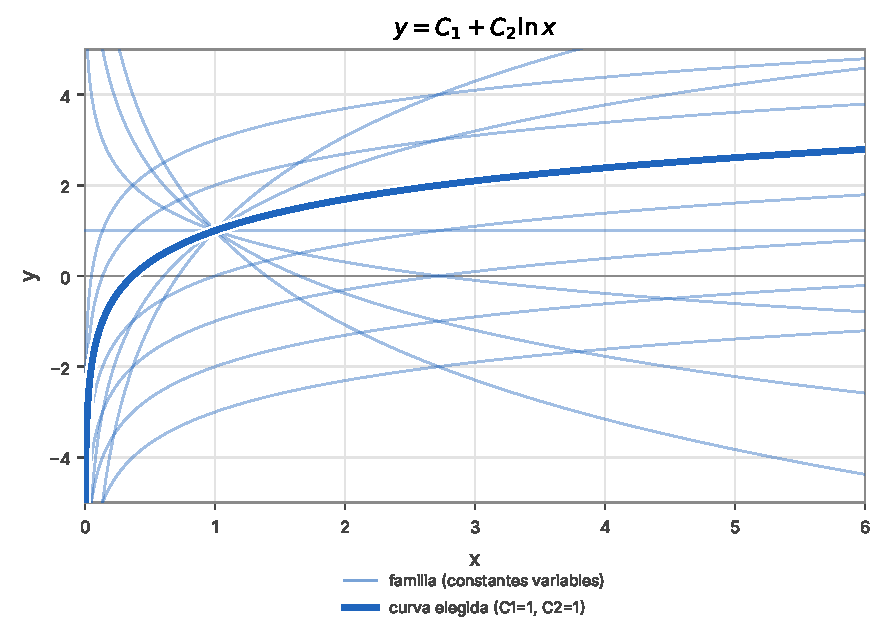
\includegraphics[width=0.8\linewidth]{h4-01.pdf}
\end{center}

\noindent\textbf{2. Hallad la EDO de la familia de curvas: $\bm{y=c_1 x + c_2 x^2}$} \\
Derivamos sucesivamente dos veces respecto de $x$:
\begin{align*}
y' &= c_1 + 2c_2 x \\
y'' &= 2c_2 \implies c_2 = \frac{y''}{2} \implies c_1 = y' - 2c_2 x = y' - x y''
\end{align*}
Despejamos
\begin{align*}
y = (y' - x y'')x + \left(\frac{y''}{2}\right)x^2 = x y' - \frac{1}{2}x^2 y'' \implies x^2 y'' - 2x y' + 2y = 0
\end{align*}
\[
\boxed{x^2 y'' - 2x y' + 2y = 0}
\]



\begin{center}
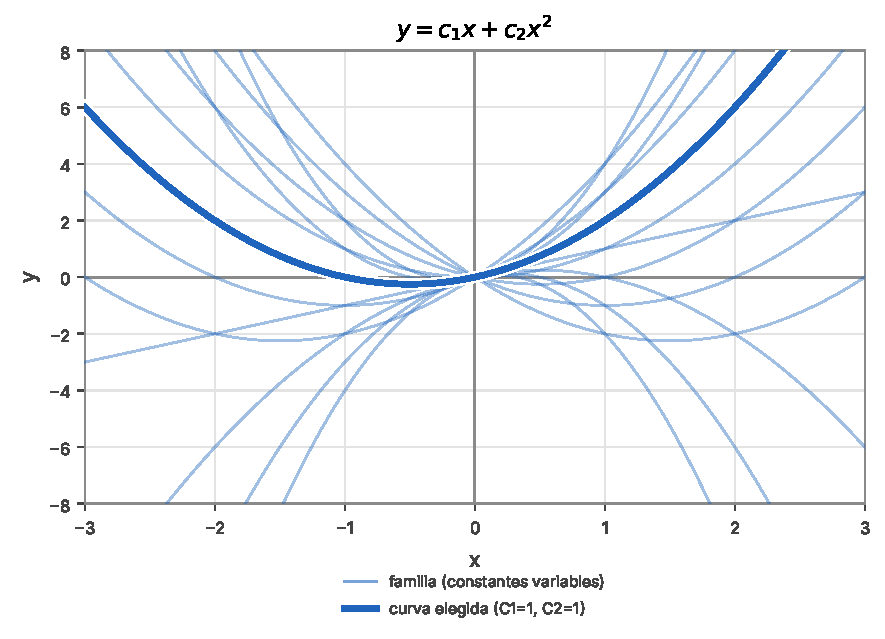
\includegraphics[width=0.8\linewidth]{h4-02.pdf}
\end{center}

\noindent\textbf{3. Hallad la EDO de la familia de curvas: $\bm{y=c_1 e^{kx} + c_2 e^{-kx}}$} \\
\begin{align*}
y' &= k c_1 e^{kx} - k c_2 e^{-kx} \\
y'' &= k^2 c_1 e^{kx} + k^2 c_2 e^{-kx} = k^2 (c_1 e^{kx} + c_2 e^{-kx}) = k^2 y
\end{align*}
\[
\boxed{y'' - k^2 y = 0}
\]



\begin{center}
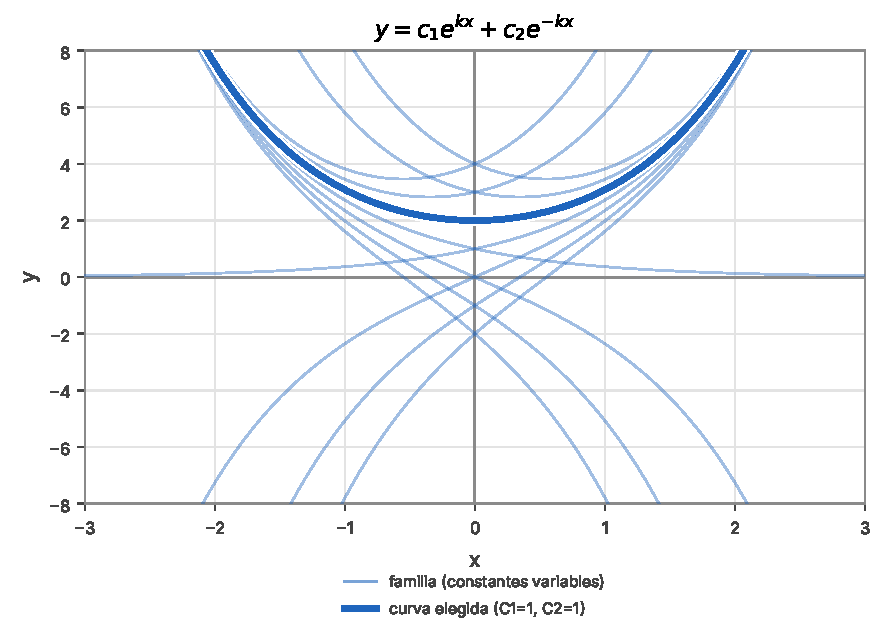
\includegraphics[width=0.8\linewidth]{h4-03.pdf}
\end{center}

\noindent\textbf{4. Hallad la EDO de la familia de curvas: $\bm{y=c_1 x + c_2 \sin x}$} \\
\begin{align*}
y' &= c_1 + c_2 \cos x \\
y'' &= -c_2 \sin x \implies c_2 = -\frac{y''}{\sin x} \\
c_1 x &= y - c_2 \sin x = y + y'' \implies c_1 = \frac{y + y''}{x} \\
\end{align*}
\begin{align*}
y' = \frac{y + y''}{x} - y'' \cot x \implies x \sin x \cdot y' = \sin x (y + y'') - x \cos x \cdot y''
\end{align*}
Reordenando términos:
\[
\boxed{(x \cos x - \sin x) y'' + x \sin x \cdot y' - y \sin x = 0}
\]



\begin{center}
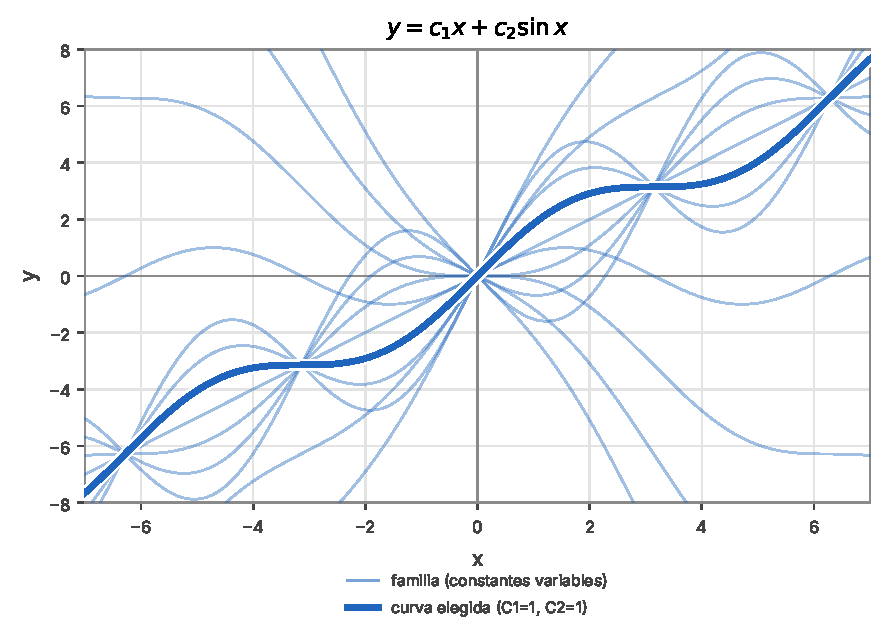
\includegraphics[width=0.8\linewidth]{h4-04.pdf}
\end{center}

\noindent\textbf{5. Si $\bm{y_1}$ e $\bm{y_2}$ son dos soluciones de una EDO lineal homogénea de segundo orden sobre $\bm{[a,b]}$ que tienen un cero común en ese intervalo, demostrad que una es múltiplo de la otra.} \\
Sea $x_0 \in [a,b]$ tal que $y_1(x_0) = y_2(x_0) = 0$. Evaluamos el Wronskiano en $x_0$:
\begin{align*}
W(y_1, y_2)(x_0) = y_1(x_0)y_2'(x_0) - y_1'(x_0)y_2(x_0) = 0 \cdot y_2'(x_0) - y_1'(x_0) \cdot 0 = 0
\end{align*}
Por el Lema de clase, si el Wronskiano de dos soluciones se anula en un punto de $[a,b]$, es idénticamente nulo en todo el intervalo: $W(y_1, y_2)(x) \equiv 0 \quad \forall x \in [a,b]$.\\
\textit{Un Wronskiano idénticamente nulo implica que $y_1$ e $y_2$ son linealmente dependientes en $[a,b]$, por lo que existe una constante $C$ tal que $y_2(x) = C y_1(x)$ o $y_1(x) = C y_2(x)$.} \quad $\blacksquare$\\


\noindent\textbf{6. Demostrad que $\bm{e^x}$ y $\bm{e^{-x}}$ son soluciones linealmente independientes de $\bm{y''-y=0}$ sobre cualquier intervalo cerrado.} \\
$y_1 = e^x \implies y_1'' = e^x \implies e^x - e^x = 0$, y $y_2 = e^{-x} \implies y_2'' = e^{-x} \implies e^{-x} - e^{-x} = 0$. Ambos satisfacen la EDO. \\
Calculamos el Wronskiano:
\begin{align*}
W(e^x, e^{-x}) = \begin{vmatrix} e^x & e^{-x} \\ e^x & -e^{-x} \end{vmatrix} = e^x(-e^{-x}) - e^x(e^{-x}) = -1 - 1 = -2 \neq 0 \quad \forall x \in \mathbb{R}
\end{align*}
\textit{Como $W \neq 0$ en todo intervalo cerrado $[a,b]$, $e^x$ y $e^{-x}$ son li.} \quad $\blacksquare$\\



\begin{center}
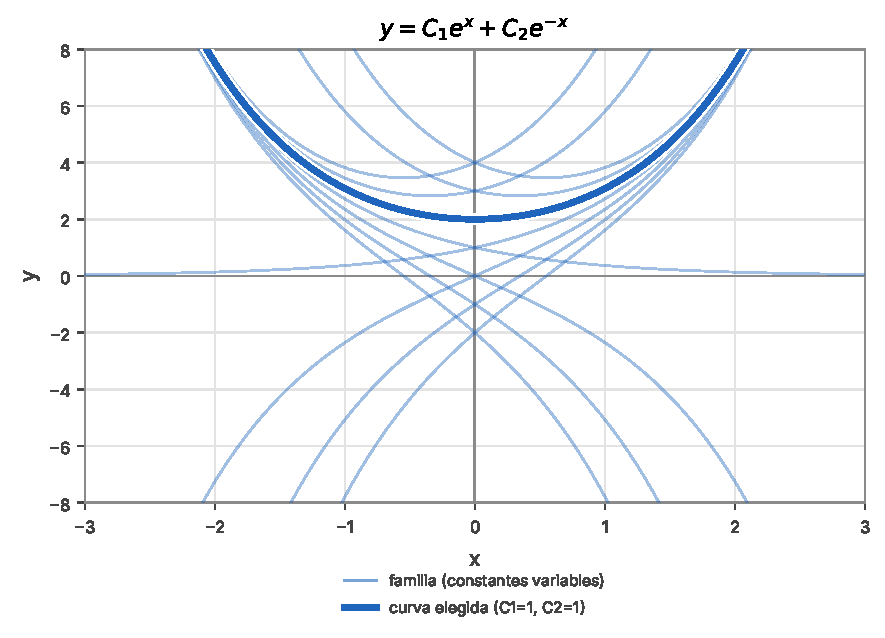
\includegraphics[width=0.8\linewidth]{h4-06.pdf}
\end{center}

\noindent\textbf{7. Comprobad que las funciones $\bm{y_1}$ e $\bm{y_2}$ son soluciones linealmente independientes de la EDO dada sobre $\bm{[0,2]}$ y hallad la solución particular:}

\begin{itemize}
\item \textbf{(a) $\bm{y''+y'-2y=0}$, $\bm{y_1=e^x}$, $\bm{y_2=e^{-2x}}$, $\bm{y(0)=8, y'(0)=2}$:}
\begin{align*}
W(e^x, e^{-2x}) = \begin{vmatrix} e^x & e^{-2x} \\ e^x & -2e^{-2x} \end{vmatrix} = -3e^{-x} \neq 0 \quad \forall x \in [0,2]
\end{align*}
$y(x) = C_1 e^x + C_2 e^{-2x}$.Con $y(0)=8 \implies C_1 + C_2 = 8$, y $y'(0)=2 \implies C_1 - 2C_2 = 2$.

\[
\boxed{y(x) = 6e^x + 2e^{-2x}}
\]


\begin{center}
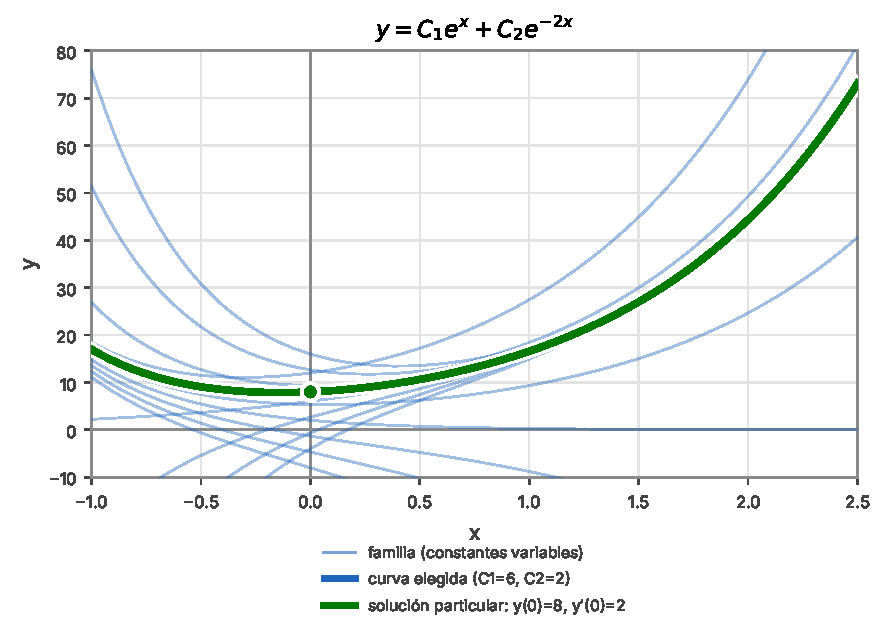
\includegraphics[width=0.8\linewidth]{h4-07-a.pdf}
\end{center}
\item \textbf{(b) $\bm{y''+y'-2y=0}$, $\bm{y_1=e^x}$, $\bm{y_2=e^{-2x}}$, $\bm{y(1)=0, y'(1)=0}$:}
\begin{align*}
\begin{cases} C_1 e + C_2 e^{-2} = 0 \\ C_1 e - 2C_2 e^{-2} = 0 \end{cases} \implies 3C_2 e^{-2} = 0 \implies C_2 = 0, C_1 = 0
\end{align*}
\[
\boxed{y(x) = 0}
\]


\begin{center}
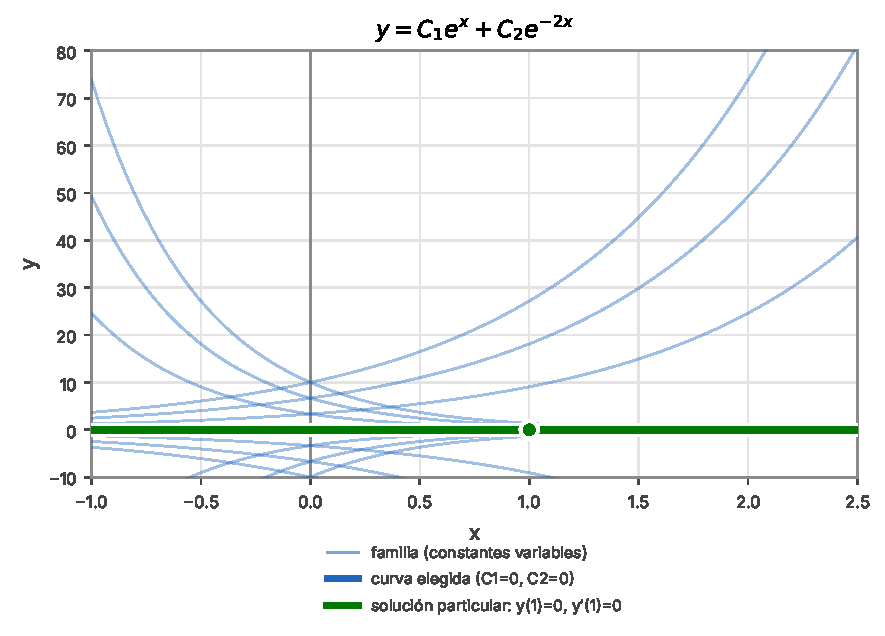
\includegraphics[width=0.8\linewidth]{h4-07-b.pdf}
\end{center}
\item \textbf{(c) $\bm{y''+5y'+6y=0}$, $\bm{y_1=e^{-2x}}$, $\bm{y_2=e^{-3x}}$, $\bm{y(0)=1, y'(0)=1}$:}\\
$y(x) = C_1 e^{-2x} + C_2 e^{-3x}$.
\begin{align*}
\begin{cases} C_1 + C_2 = 1 \\ -2C_1 - 3C_2 = 1 \end{cases} \implies C_1 = 4, \quad C_2 = -3
\end{align*}
\[
\boxed{y(x) = 4e^{-2x} - 3e^{-3x}}
\]


\begin{center}
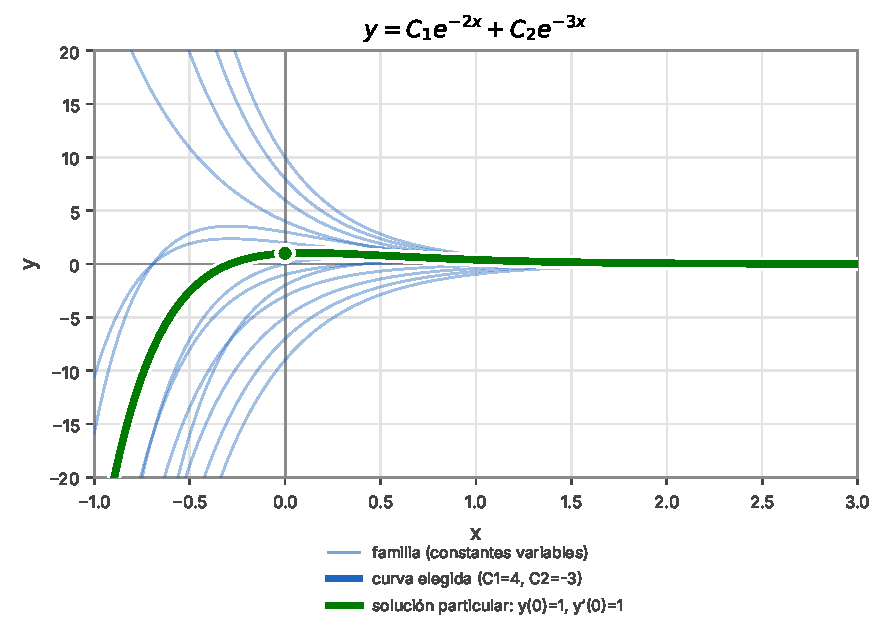
\includegraphics[width=0.8\linewidth]{h4-07-c.pdf}
\end{center}
\item \textbf{(d) $\bm{y''+y'=0}$, $\bm{y_1=1}$, $\bm{y_2=e^{-x}}$, $\bm{y(2)=0, y'(2)=1/e^2}$:}
\begin{align*}
W(1, e^{-x}) = -e^{-x} \neq 0 \quad \forall x \in [0,2]
\end{align*}
$y(x) = C_1 + C_2 e^{-x} \implies y'(x) = -C_2 e^{-x}$.\\
$y'(2) = -C_2 e^{-2} = e^{-2} \implies C_2 = -1$. \\
$y(2) = C_1 - e^{-2} = 0 \implies C_1 = e^{-2}$.\\
\[
\boxed{y(x) = e^{-2} - e^{-x}}
\]

\begin{center}
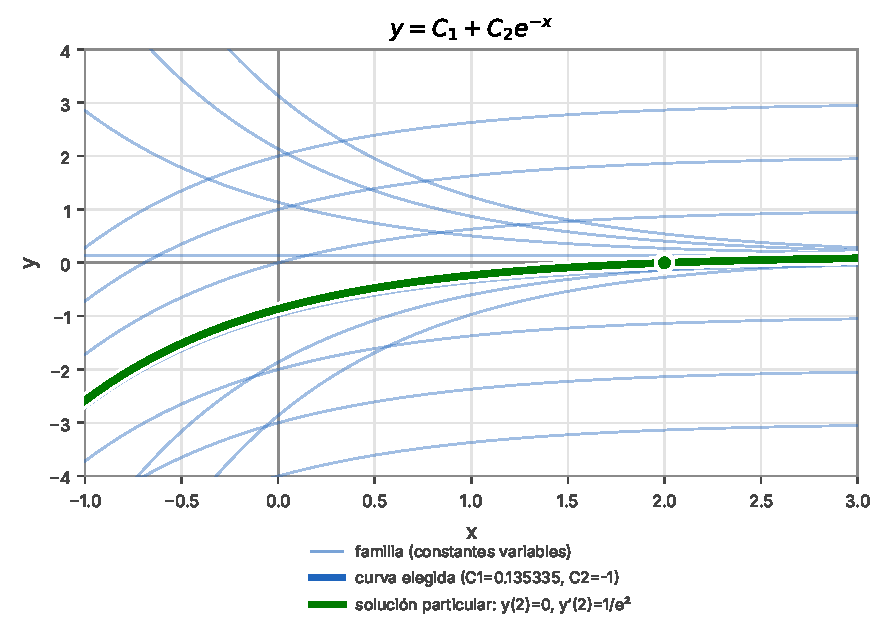
\includegraphics[width=0.8\linewidth]{h4-07-d.pdf}
\end{center}
\end{itemize}


\noindent\textbf{8. Verificad que $\bm{y_1(x)=\sin x}$ es solución de $\bm{y''+y=0}$. Obtened otra solución $\bm{y_2(x)}$ L.I. y la solución general.} \\
Comprobamos la primera solución derivando: $(\sin x)'' + \sin x = -\sin x + \sin x = 0 \quad \checkmark$. \\
La EDO es lineal homogénea con coef const,
\begin{align*}
s^2 + 1 = 0 \implies s = \pm i
\end{align*}
Las raíces imaginarias puras generan soluciones trigonométricas. Como ya conocemos $y_1(x) = \sin x$, la otra solución linealmente independiente es:
\[
y_2(x) = \cos x
\]
Por lo tanto, la solución general es:
\[
\boxed{y(x) = C_1 \sin x + C_2 \cos x}
\]



\begin{center}
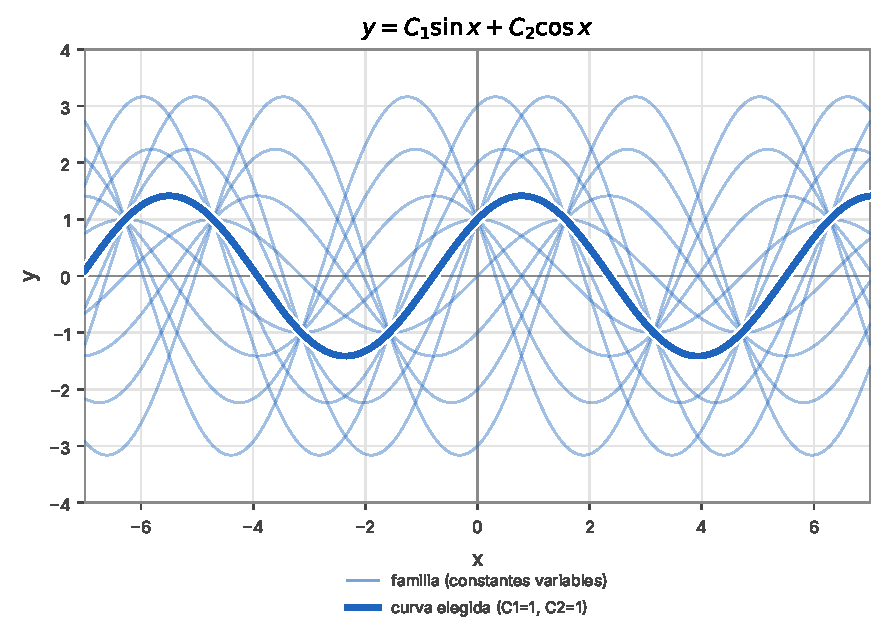
\includegraphics[width=0.8\linewidth]{h4-08.pdf}
\end{center}

\noindent\textbf{9. La EDO $\bm{xy''+3y'=0}$ admite $\bm{y_1(x)=1}$. Hallad otra solución $\bm{y_2(x)}$ L.I. sobre cualquier intervalo que no contenga $\bm{0}$ y la solución general.} \\
$p = y' \implies p' = y''$:
\begin{align*}
x p' + 3p = 0 \implies x \frac{dp}{dx} = -3p \implies \frac{dp}{p} = -\frac{3}{x} dx
\end{align*}
\begin{align*}
\ln|p| = -3\ln|x| + C \implies p(x) = \frac{K}{x^3}
\end{align*}
\begin{align*}
y(x) = \int \frac{K}{x^3} dx = -\frac{K}{2x^2} + C_1 = \frac{C_2}{x^2} + C_1
\end{align*}
\begin{align*}
W(1, x^{-2}) = -2x^{-3} \neq 0 \quad \text{para } x \neq 0
\end{align*}
\[
\boxed{y(x) = C_1 + \frac{C_2}{x^2}}
\]



\begin{center}
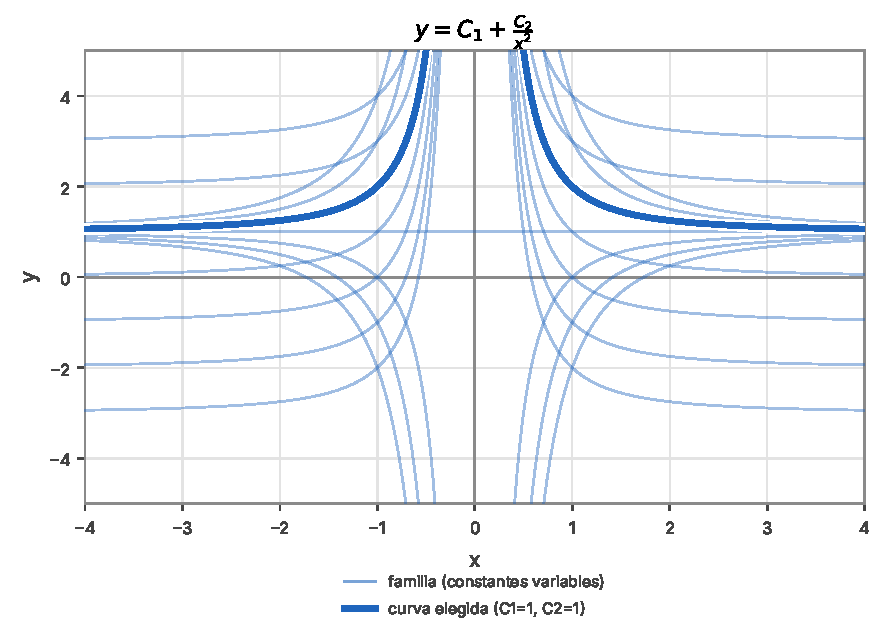
\includegraphics[width=0.8\linewidth]{h4-09.pdf}
\end{center}

\noindent\textbf{10. Comprobad que $\bm{y_1(x)=e^x}$ es solución de $\bm{xy''-(2x+1)y'+(x+1)y=0}$ y hallad la solución general.} \\
Sustituyendo $y_1 = e^x \implies y_1' = e^x, \, y_1'' = e^x$:
\begin{align*}
x e^x - (2x+1)e^x + (x+1)e^x = e^x(x - 2x - 1 + x + 1) = 0 \quad \checkmark
\end{align*}
$y_2(x) = v(x) e^x \implies y_2' = (v'+v)e^x, \, y_2'' = (v''+2v'+v)e^x$.
\begin{align*}
x(v''+2v'+v)e^x - (2x+1)(v'+v)e^x + (x+1)v e^x &= 0 \\
x v'' + [2x - (2x+1)] v' &= 0 \implies x v'' - v' = 0 \implies \frac{v''}{v'} = \frac{1}{x}
\end{align*}
$\ln v' = \ln x \implies v' = x \implies v(x) = \frac{x^2}{2} \implies y_2(x) = x^2 e^x$.
\[
\boxed{y(x) = C_1 e^x + C_2 x^2 e^x}
\]



\begin{center}
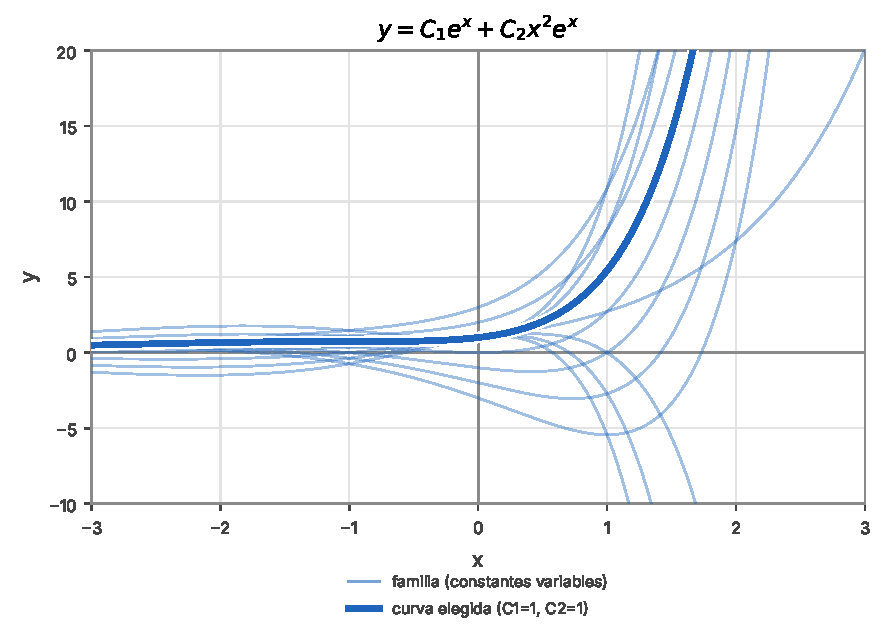
\includegraphics[width=0.8\linewidth]{h4-10.pdf}
\end{center}

\noindent\textbf{11. Hallad la solución general de las siguientes ecuaciones:}

\begin{itemize}
\item \textbf{(a) $\bm{y''-4y'+4y=0}$:} $(s-2)^2 = 0 \implies s = 2$ (doble). $\quad \boxed{y(x) = (C_1 + C_2 x)e^{2x}}$

\begin{center}
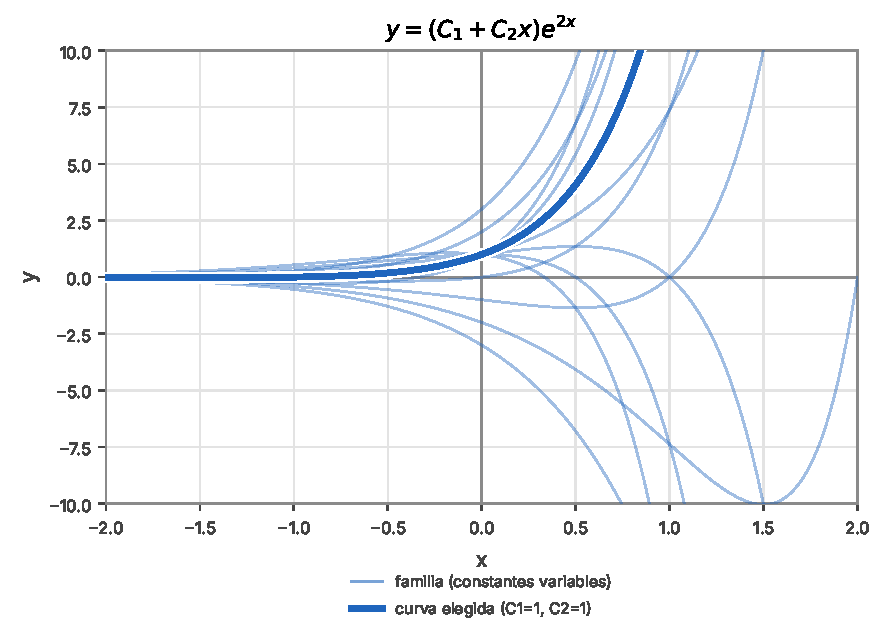
\includegraphics[width=0.8\linewidth]{h4-11-a.pdf}
\end{center}
\item \textbf{(b) $\bm{y''-9y'+20y=0}$:} $(s-4)(s-5) = 0 \implies s_1 = 4, s_2 = 5$. $\quad \boxed{y(x) = C_1 e^{4x} + C_2 e^{5x}}$

\begin{center}
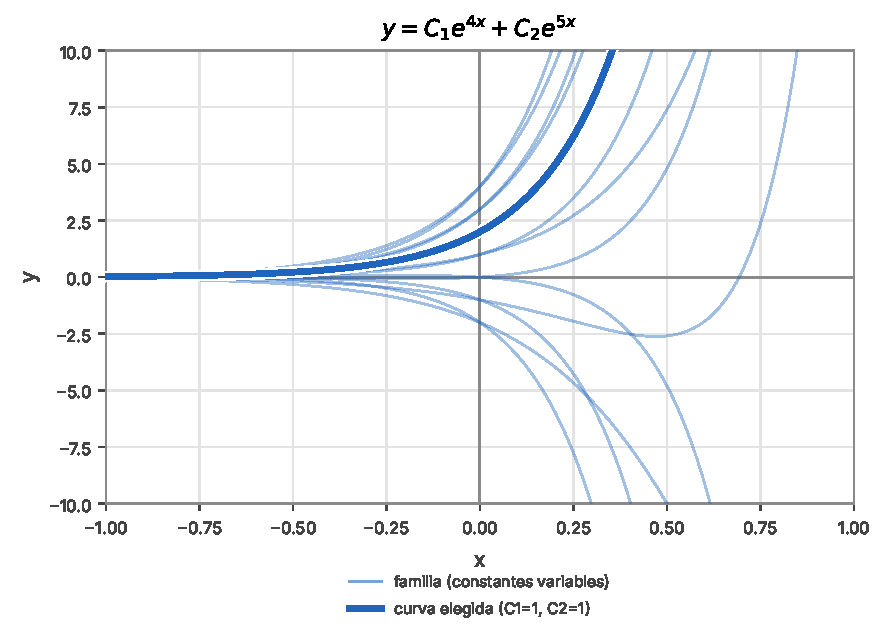
\includegraphics[width=0.8\linewidth]{h4-11-b.pdf}
\end{center}
\item \textbf{(c) $\bm{2y''+2y'+3y=0}$:} $s = -\frac{1}{2} \pm i\frac{\sqrt{5}}{2}$. $\quad \boxed{y(x) = e^{-x/2}\left(C_1 \cos\frac{\sqrt{5}}{2}x + C_2 \sin\frac{\sqrt{5}}{2}x\right)}$

\begin{center}
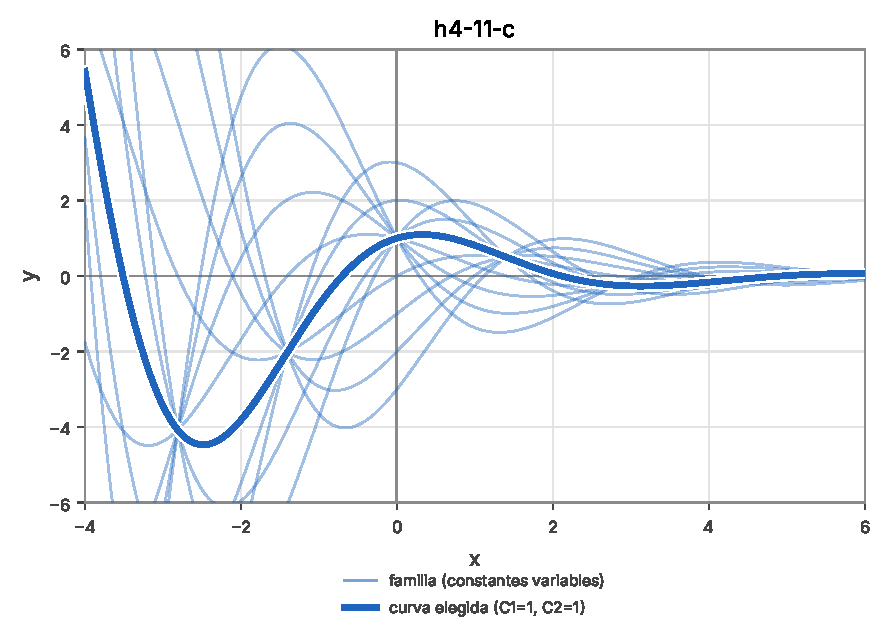
\includegraphics[width=0.8\linewidth]{h4-11-c.pdf}
\end{center}
\item \textbf{(d) $\bm{4y''-12y'+9y=0}$:} $(2s-3)^2 = 0 \implies s = 3/2$ (doble). $\quad \boxed{y(x) = (C_1 + C_2 x)e^{3x/2}}$

\begin{center}
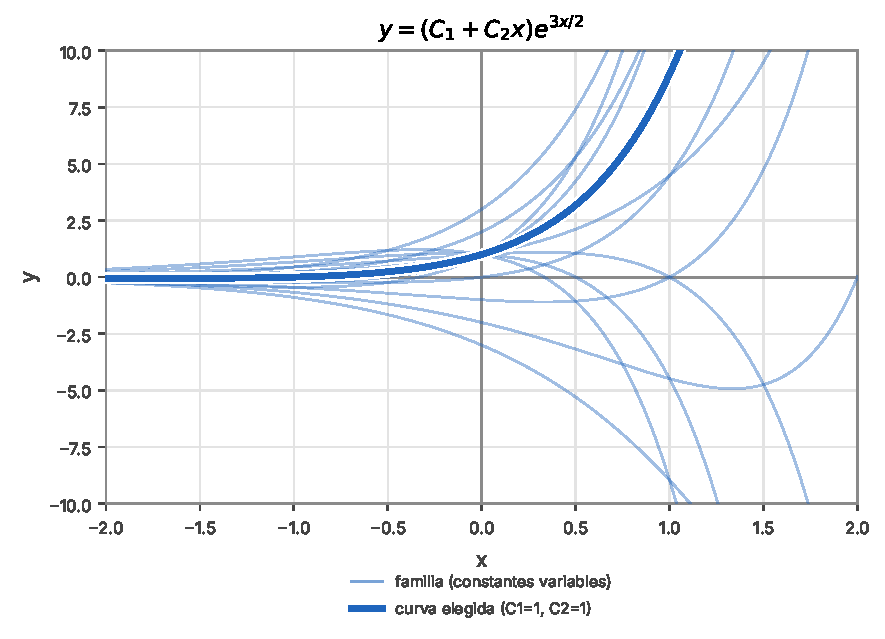
\includegraphics[width=0.8\linewidth]{h4-11-d.pdf}
\end{center}
\item \textbf{(e) $\bm{y''+y'=0}$:} $s(s+1) = 0 \implies s_1 = 0, s_2 = -1$. $\quad \boxed{y(x) = C_1 + C_2 e^{-x}}$

\begin{center}
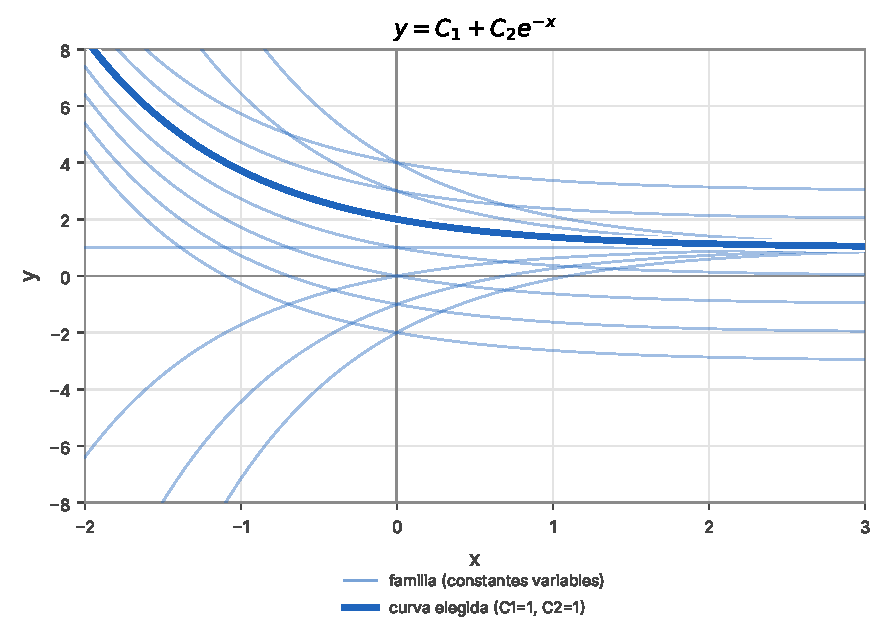
\includegraphics[width=0.8\linewidth]{h4-11-e.pdf}
\end{center}
\item \textbf{(f) $\bm{y''-6y'+25y=0}$:} $s = 3 \pm 4i$. $\quad \boxed{y(x) = e^{3x}(C_1 \cos 4x + C_2 \sin 4x)}$

\begin{center}
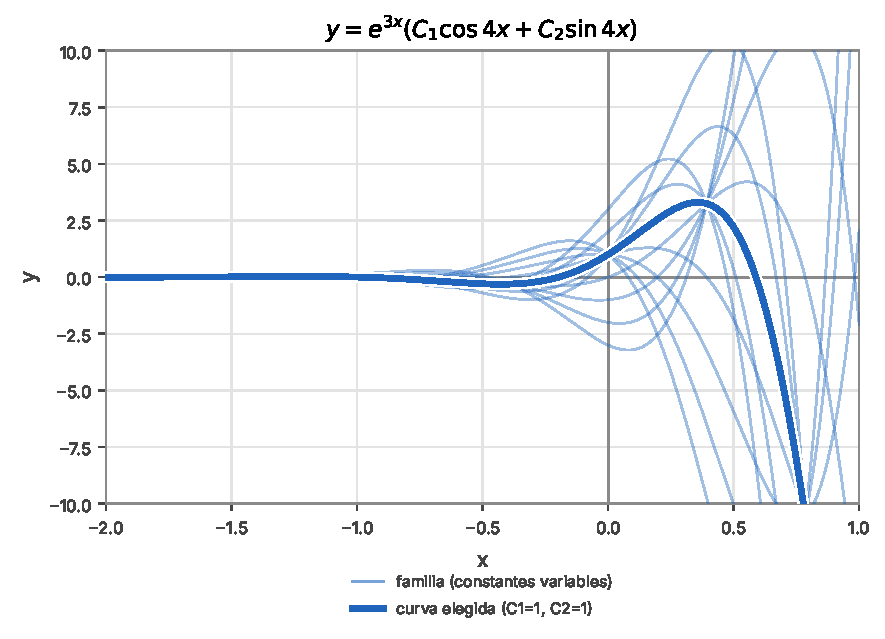
\includegraphics[width=0.8\linewidth]{h4-11-f.pdf}
\end{center}
\item \textbf{(g) $\bm{4y''+20y'+25y=0}$:} $(2s+5)^2 = 0 \implies s = -5/2$ (doble). $\quad \boxed{y(x) = (C_1 + C_2 x)e^{-5x/2}}$

\begin{center}
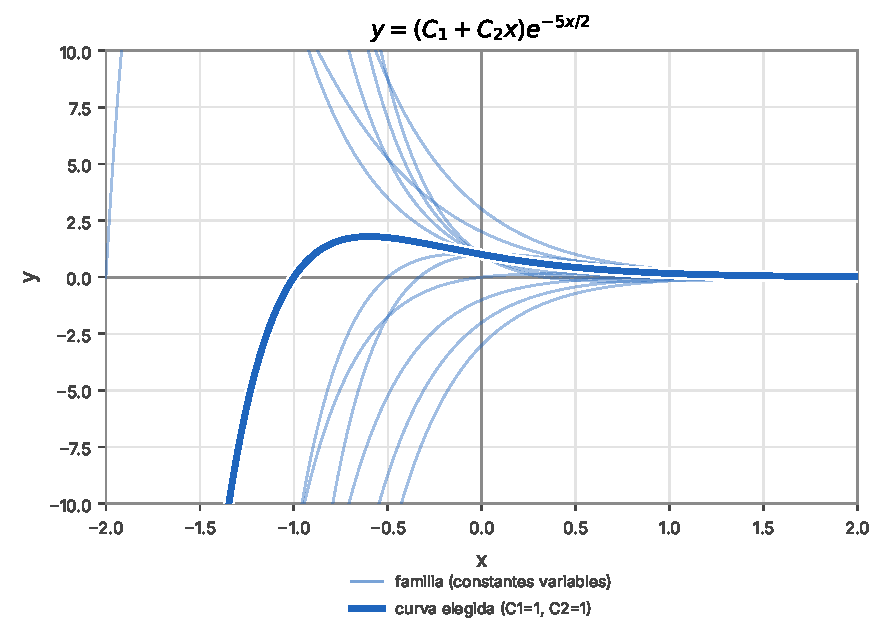
\includegraphics[width=0.8\linewidth]{h4-11-g.pdf}
\end{center}
\item \textbf{(h) $\bm{y''+2y'+3y=0}$:} $s = -1 \pm i\sqrt{2}$. $\quad \boxed{y(x) = e^{-x}(C_1 \cos\sqrt{2}x + C_2 \sin\sqrt{2}x)}$

\begin{center}
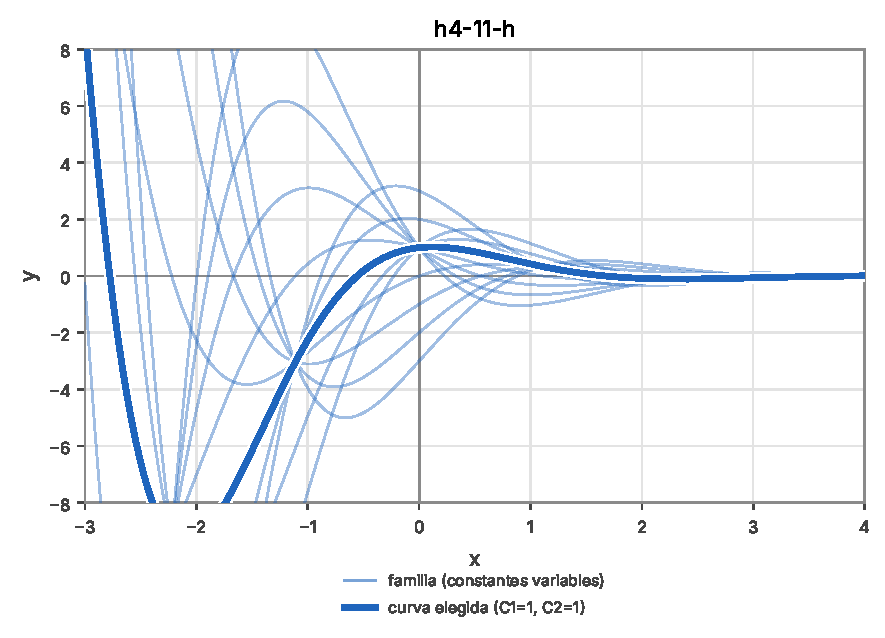
\includegraphics[width=0.8\linewidth]{h4-11-h.pdf}
\end{center}
\item \textbf{(i) $\bm{y''=4y}$:} $s^2 - 4 = 0 \implies s = \pm 2$. $\quad \boxed{y(x) = C_1 e^{2x} + C_2 e^{-2x}}$

\begin{center}
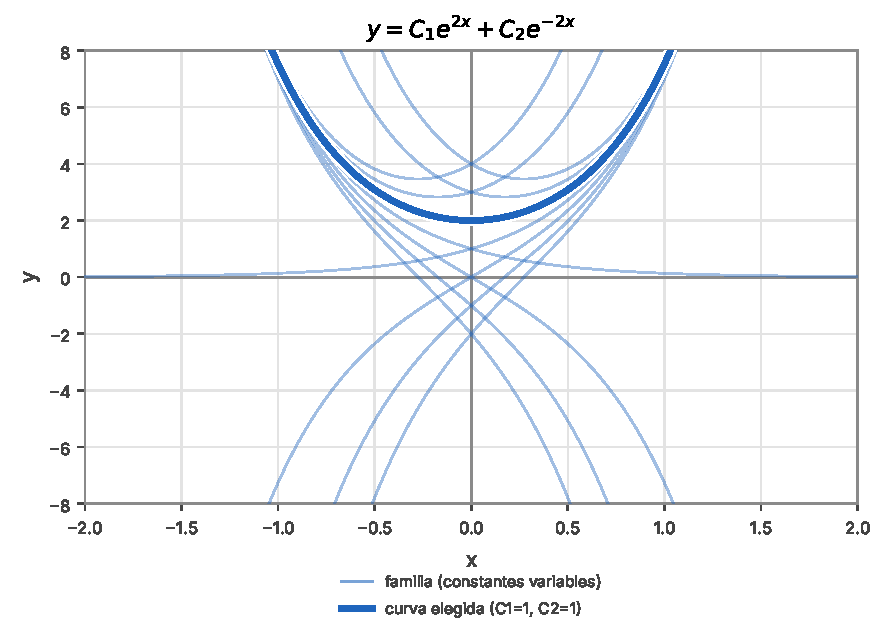
\includegraphics[width=0.8\linewidth]{h4-11-i.pdf}
\end{center}
\item \textbf{(j) $\bm{4y''-8y'+7y=0}$:} $s = 1 \pm i\frac{\sqrt{3}}{2}$. $\quad \boxed{y(x) = e^x\left(C_1 \cos\frac{\sqrt{3}}{2}x + C_2 \sin\frac{\sqrt{3}}{2}x\right)}$

\begin{center}
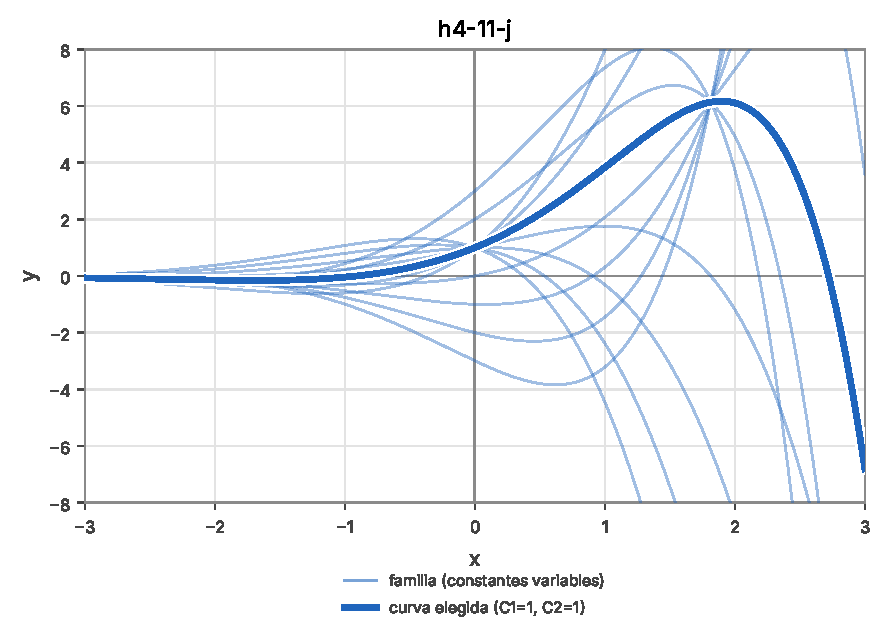
\includegraphics[width=0.8\linewidth]{h4-11-j.pdf}
\end{center}
\item \textbf{(k) $\bm{2y''+y'-y=0}$:} $(2s-1)(s+1) = 0 \implies s_1 = 1/2, s_2 = -1$. $\quad \boxed{y(x) = C_1 e^{x/2} + C_2 e^{-x}}$

\begin{center}
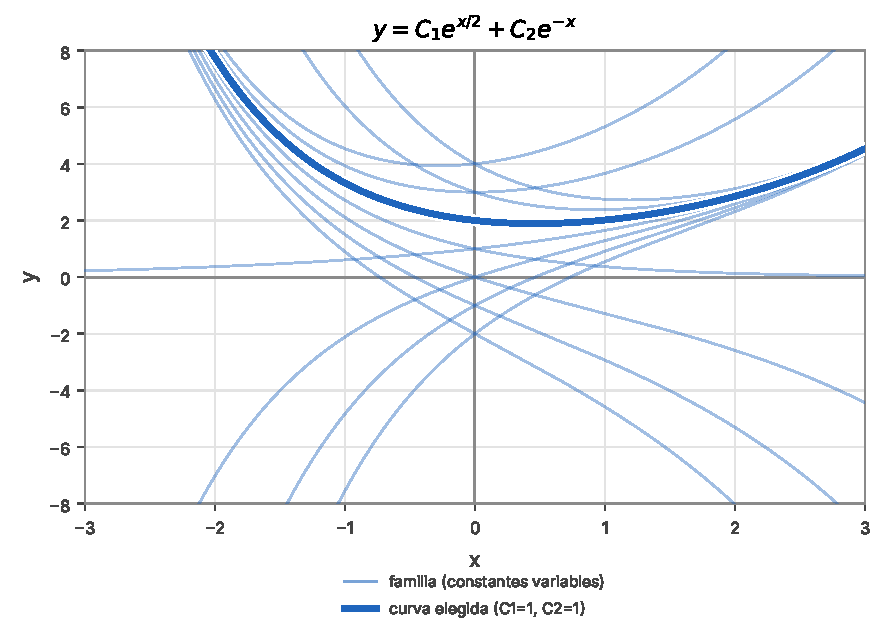
\includegraphics[width=0.8\linewidth]{h4-11-k.pdf}
\end{center}
\item \textbf{(l) $\bm{16y''-8y'+y=0}$:} $(4s-1)^2 = 0 \implies s = 1/4$ (doble). $\quad \boxed{y(x) = (C_1 + C_2 x)e^{x/4}}$

\begin{center}
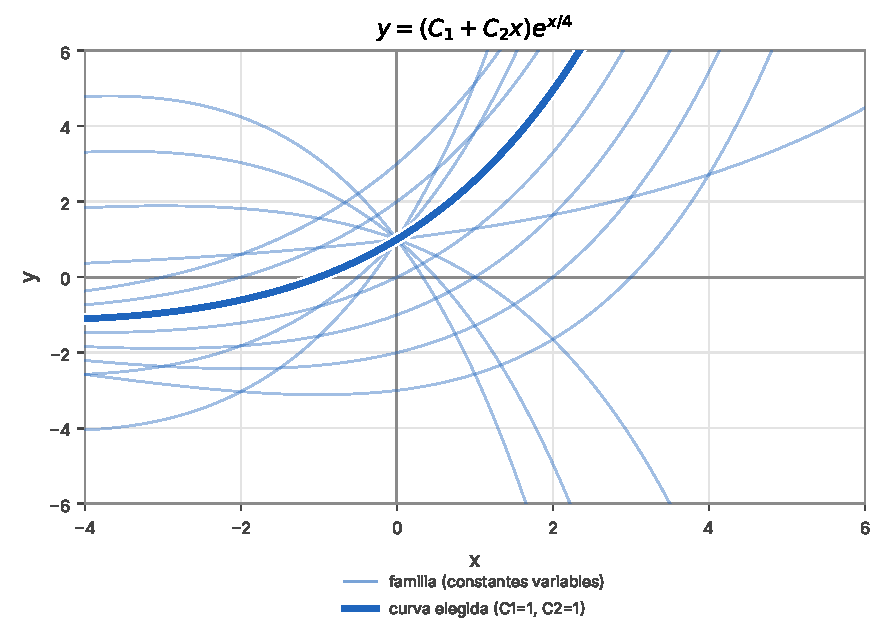
\includegraphics[width=0.8\linewidth]{h4-11-l.pdf}
\end{center}
\item \textbf{(m) $\bm{y''+4y'+5y=0}$:} $s = -2 \pm i$. $\quad \boxed{y(x) = e^{-2x}(C_1 \cos x + C_2 \sin x)}$

\begin{center}
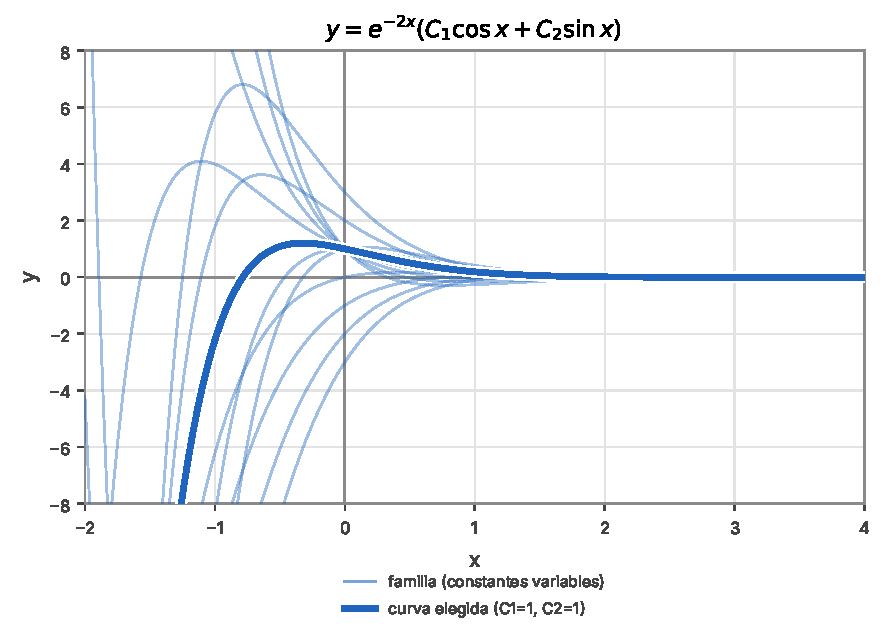
\includegraphics[width=0.8\linewidth]{h4-11-m.pdf}
\end{center}
\item \textbf{(n) $\bm{y''+4y'-5y=0}$:} $(s+5)(s-1) = 0 \implies s_1 = 1, s_2 = -5$. $\quad \boxed{y(x) = C_1 e^x + C_2 e^{-5x}}$\\

\begin{center}
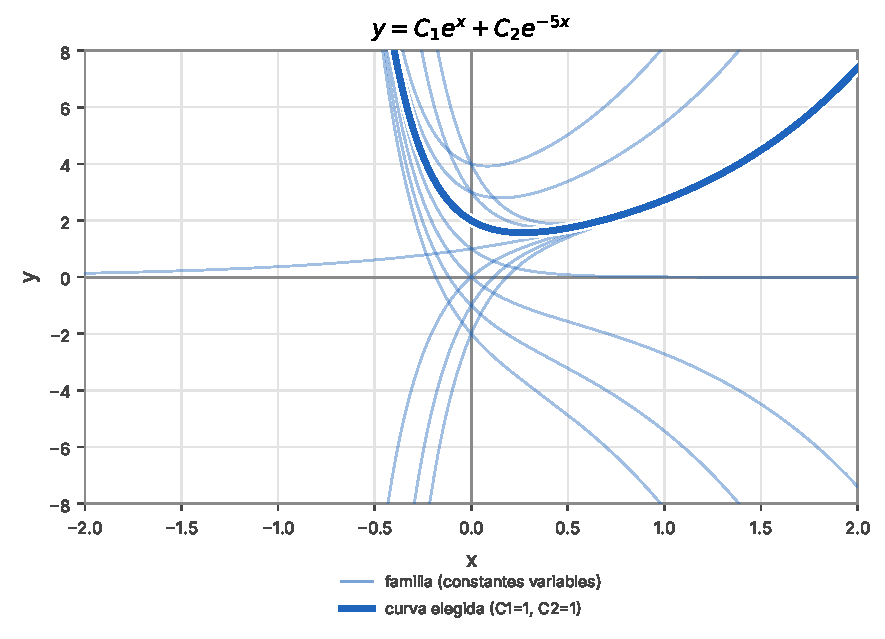
\includegraphics[width=0.8\linewidth]{h4-11-n.pdf}
\end{center}
\end{itemize}

\noindent\textbf{12. Resolved los siguientes problemas con condiciones iniciales:}

\begin{itemize}
\item \textbf{(a) $\bm{y''-5y'+6y=0}$ con $\bm{y(1)=e^2, y'(1)=3e^2}$:} \\
$y(x) = C_1 e^{2x} + C_2 e^{3x}$. Evaluando en $x=1$:
\begin{align*}
\begin{cases} C_1 e^2 + C_2 e^3 = e^2 \\ 2C_1 e^2 + 3C_2 e^3 = 3e^2 \end{cases} \implies C_1 = 0, \quad C_2 = e^{-1}
\end{align*}
\[
\boxed{y(x) = e^{3x-1}}
\]


\begin{center}
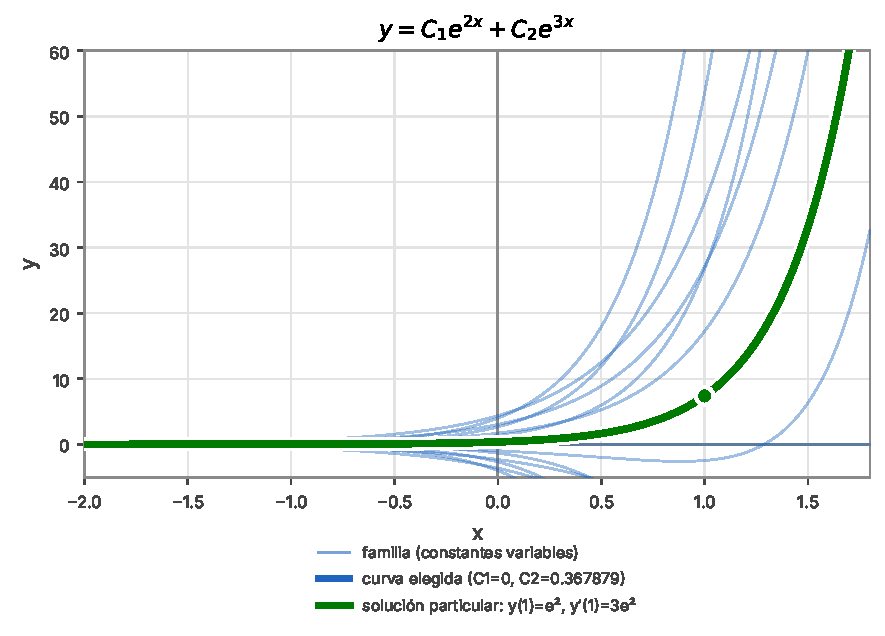
\includegraphics[width=0.8\linewidth]{h4-12-a.pdf}
\end{center}
\item \textbf{(b) $\bm{y''-6y'+5y=0}$ con $\bm{y(0)=3, y'(0)=11}$:} \\
$y(x) = C_1 e^x + C_2 e^{5x}$.
\begin{align*}
\begin{cases} C_1 + C_2 = 3 \\ C_1 + 5C_2 = 11 \end{cases} \implies 4C_2 = 8 \implies C_2 = 2, \quad C_1 = 1
\end{align*}
\[
\boxed{y(x) = e^x + 2e^{5x}}
\]


\begin{center}
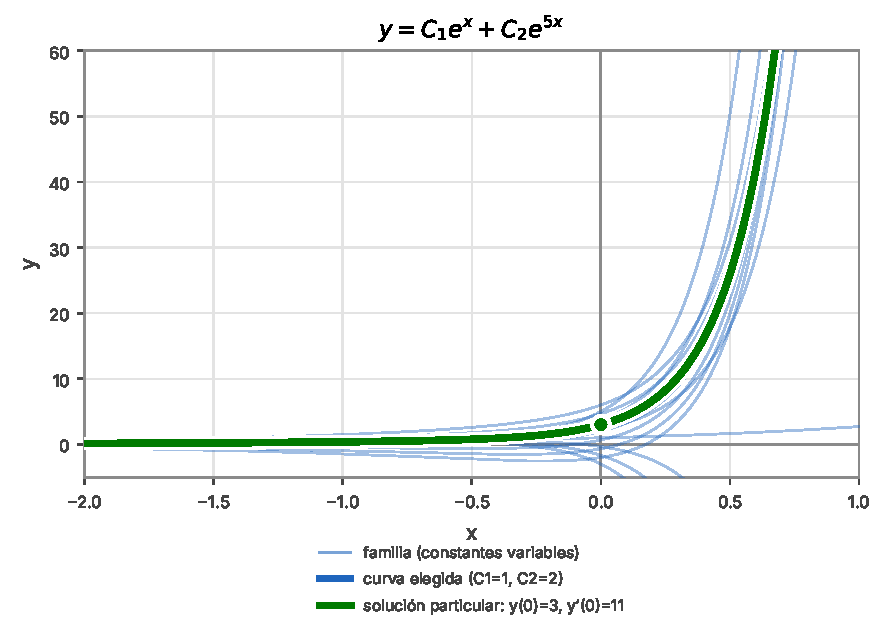
\includegraphics[width=0.8\linewidth]{h4-12-b.pdf}
\end{center}
\item \textbf{(c) $\bm{y''-6y'+9y=0}$ con $\bm{y(0)=0, y'(0)=5}$:} \\
$y(x) = (C_1 + C_2 x)e^{3x} \implies y(0) = C_1 = 0$. $y'(x) = C_2 e^{3x} + 3C_2 x e^{3x} \implies y'(0) = C_2 = 5$.
\[
\boxed{y(x) = 5x e^{3x}}
\]


\begin{center}
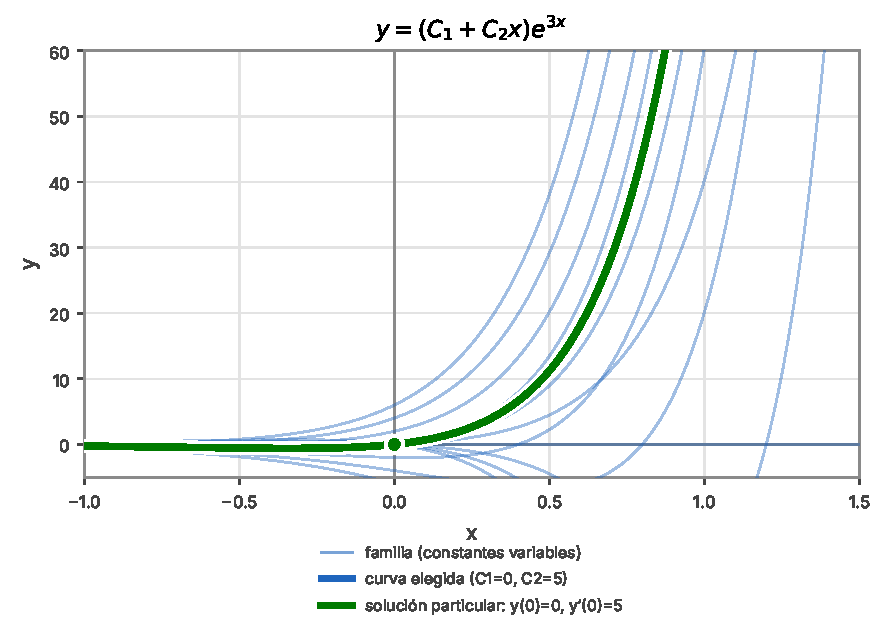
\includegraphics[width=0.8\linewidth]{h4-12-c.pdf}
\end{center}
\item \textbf{(d) $\bm{y''+4y'+5y=0}$ con $\bm{y(0)=1, y'(0)=0}$:} \\
$y(x) = e^{-2x}(C_1 \cos x + C_2 \sin x) \implies y(0) = C_1 = 1$. \\
$y'(0) = -2C_1 + C_2 = 0 \implies C_2 = 2$.
\[
\boxed{y(x) = e^{-2x}(\cos x + 2\sin x)}
\]


\begin{center}
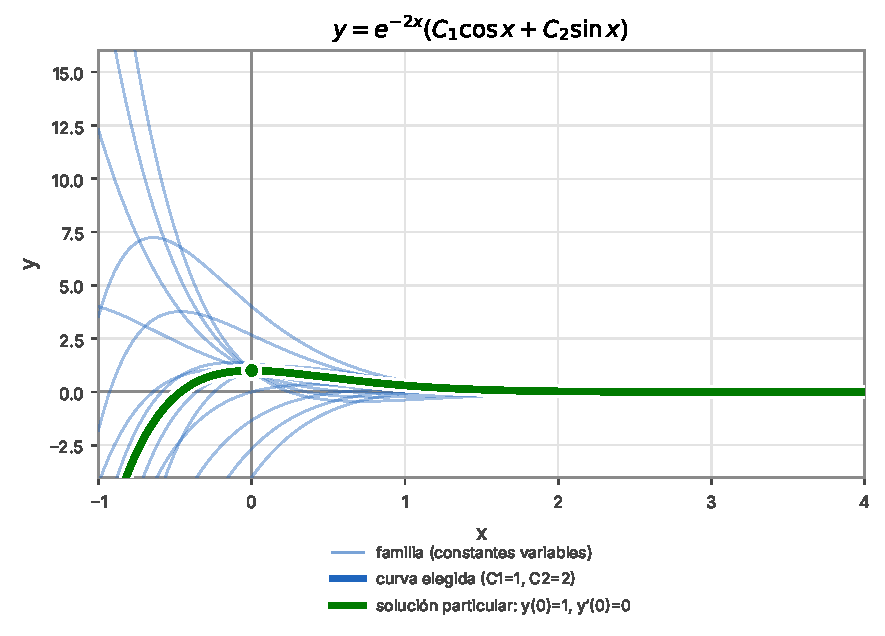
\includegraphics[width=0.8\linewidth]{h4-12-d.pdf}
\end{center}
\item \textbf{(e) $\bm{y''+4y'+2y=0}$ con $\bm{y(0)=-1, y'(0)=2+3\sqrt{2}}$:} \\
$s = -2 \pm \sqrt{2} \implies y(x) = C_1 e^{(-2+\sqrt{2})x} + C_2 e^{(-2-\sqrt{2})x}$.
\begin{align*}
\begin{cases} C_1 + C_2 = -1 \\ (-2+\sqrt{2})C_1 + (-2-\sqrt{2})C_2 = 2+3\sqrt{2} \end{cases} \implies C_1 = 1, \quad C_2 = -2
\end{align*}
\[
\boxed{y(x) = e^{(-2+\sqrt{2})x} - 2e^{(-2-\sqrt{2})x}}
\]


\begin{center}
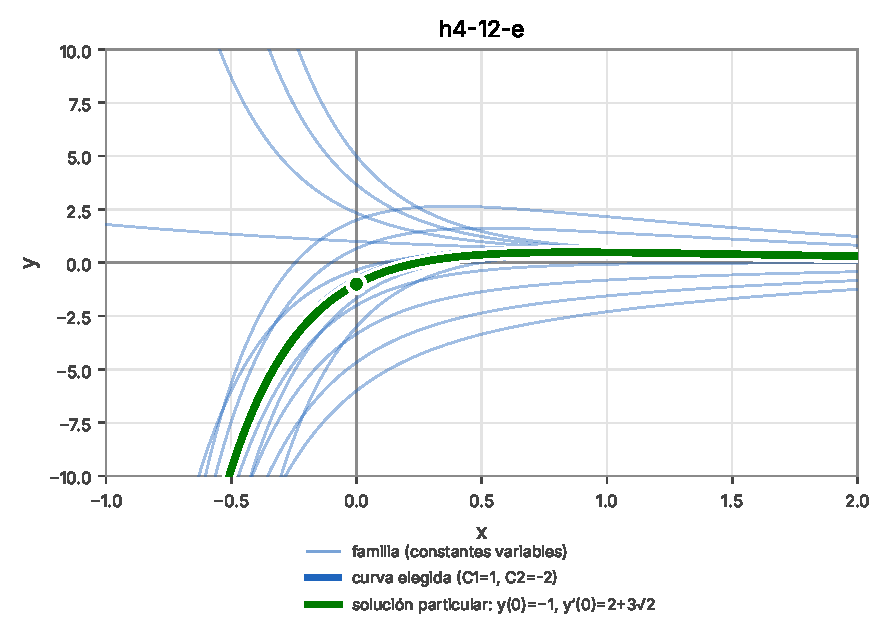
\includegraphics[width=0.8\linewidth]{h4-12-e.pdf}
\end{center}
\item \textbf{(f) $\bm{y''+8y'-9y=0}$ con $\bm{y(1)=2, y'(1)=0}$:} \\
$y(x) = C_1 e^x + C_2 e^{-9x}$.
\begin{align*}
\begin{cases} C_1 e + C_2 e^{-9} = 2 \\ C_1 e - 9C_2 e^{-9} = 0 \end{cases} \implies 10C_2 e^{-9} = 2 \implies C_2 = \frac{e^9}{5}, \quad C_1 = \frac{9}{5e}
\end{align*}
\[
\boxed{y(x) = \frac{9}{5}e^{x-1} + \frac{1}{5}e^{-9(x-1)}}
\]

\begin{center}
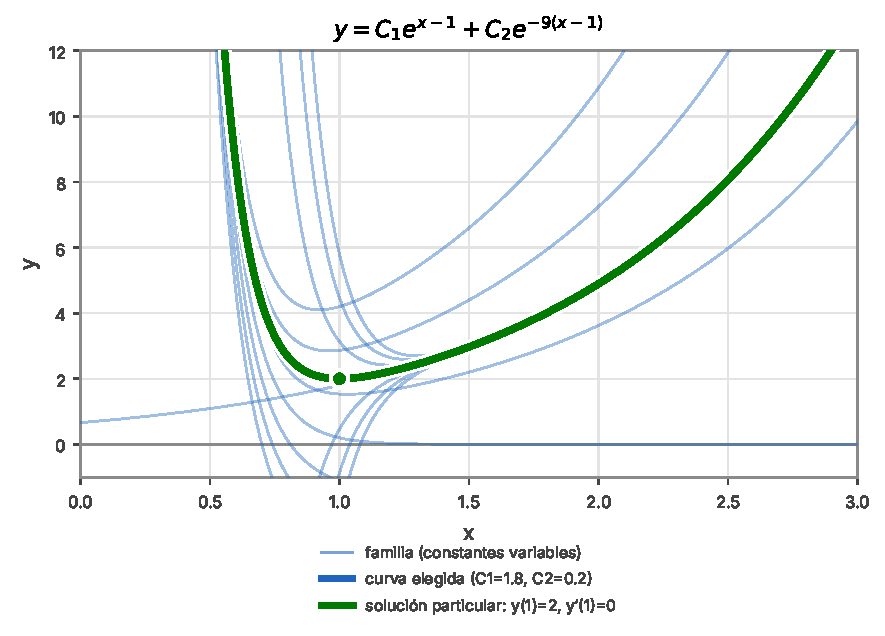
\includegraphics[width=0.8\linewidth]{h4-12-f.pdf}
\end{center}
\end{itemize}

\noindent\textbf{13. Ecuación equidimensional de Euler: $\bm{x^2y''+pxy'+qy=0}$. Demostrad que $\bm{x=e^z}$ la transforma en coeficientes constantes y aplicadla:} \\
Demostración: $z = \ln x \implies \frac{dz}{dx} = \frac{1}{x}$.
\begin{align*}
y' &= \frac{dy}{dz}\frac{dz}{dx} = \frac{1}{x}\frac{dy}{dz} \implies x y' = \frac{dy}{dz} \\
y'' &= \frac{d}{dx}\left(\frac{1}{x}\frac{dy}{dz}\right) = -\frac{1}{x^2}\frac{dy}{dz} + \frac{1}{x^2}\frac{d^2y}{dz^2} \implies x^2 y'' = \frac{d^2y}{dz^2} - \frac{dy}{dz}
\end{align*}
Sustituyendo en la EDO: $\frac{d^2y}{dz^2} + (p-1)\frac{dy}{dz} + qy = 0$, con coeficientes constantes. \quad $\blacksquare$

\begin{itemize}
\item \textbf{(a) $\bm{4x^2y''-3y=0}$:} $s(s-1) - 3/4 = 0 \implies s_1 = 3/2, s_2 = -1/2$. $\quad \boxed{y(x) = C_1 x^{3/2} + C_2 x^{-1/2}}$

\begin{center}
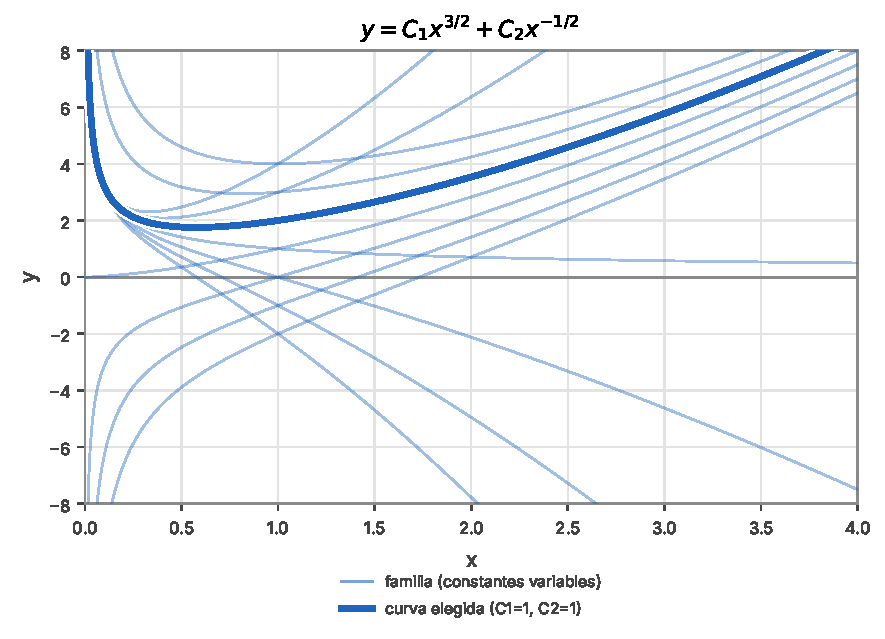
\includegraphics[width=0.8\linewidth]{h4-13-a.pdf}
\end{center}
\item \textbf{(b) $\bm{x^2y''-3xy'+4y=0}$:} $s(s-1) - 3s + 4 = (s-2)^2 = 0$. $\quad \boxed{y(x) = (C_1 + C_2 \ln x)x^2}$

\begin{center}
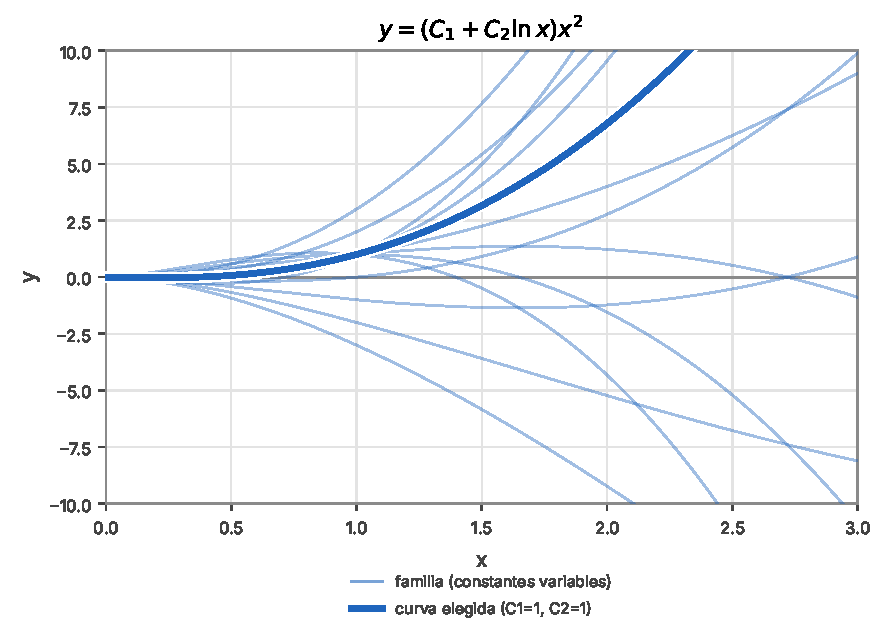
\includegraphics[width=0.8\linewidth]{h4-13-b.pdf}
\end{center}
\item \textbf{(c) $\bm{x^2y''+2xy'-6y=0}$:} $s(s-1) + 2s - 6 = (s+3)(s-2) = 0$. $\quad \boxed{y(x) = C_1 x^2 + C_2 x^{-3}}$

\begin{center}
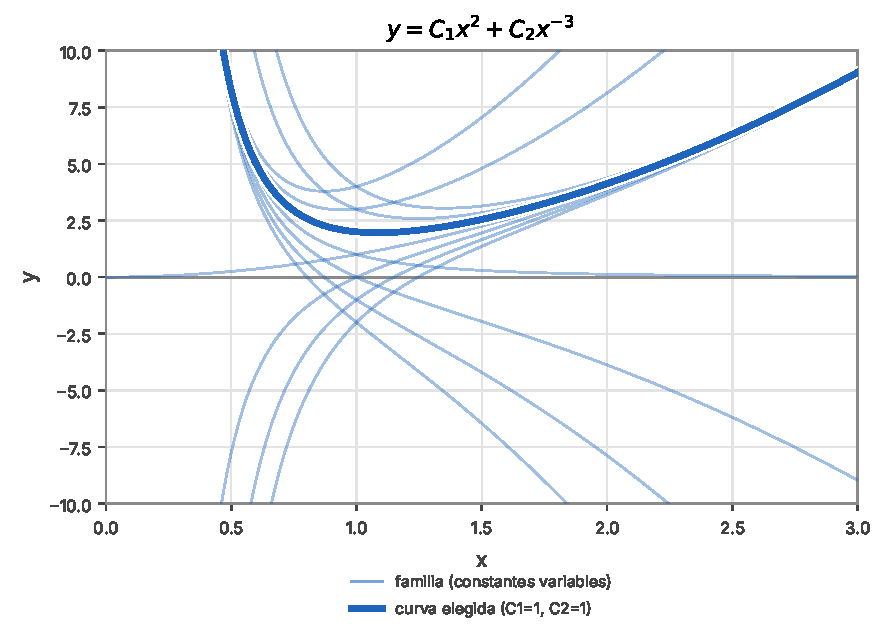
\includegraphics[width=0.8\linewidth]{h4-13-c.pdf}
\end{center}
\item \textbf{(d) $\bm{x^2y''+2xy'+3y=0}$:} $s^2 + s + 3 = 0 \implies s = -\frac{1}{2} \pm i\frac{\sqrt{11}}{2}$. \\
$\boxed{y(x) = x^{-1/2}\left(C_1 \cos\left(\frac{\sqrt{11}}{2}\ln x\right) + C_2 \sin\left(\frac{\sqrt{11}}{2}\ln x\right)\right)}$

\begin{center}
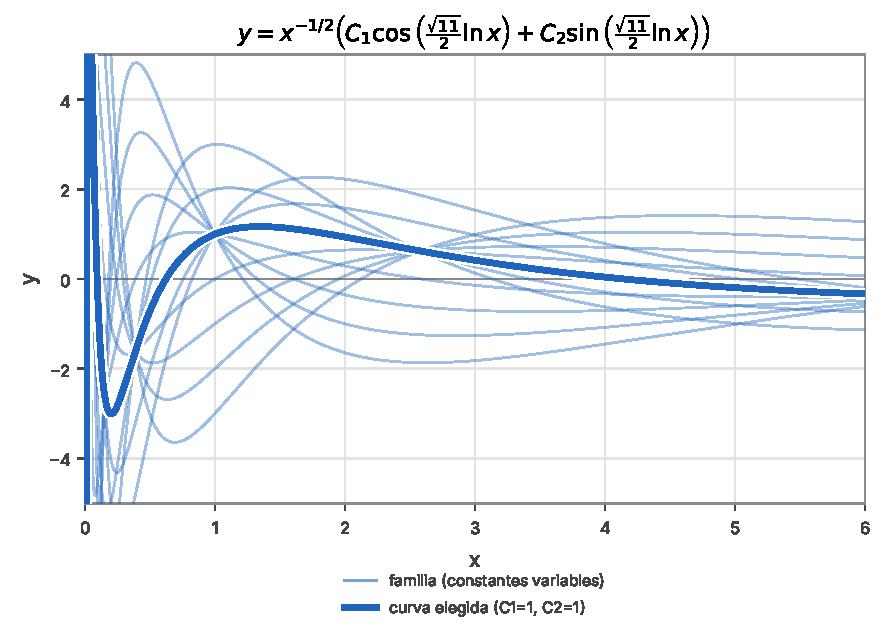
\includegraphics[width=0.8\linewidth]{h4-13-d.pdf}
\end{center}
\item \textbf{(e) $\bm{x^2y''+xy'-2y=0}$:} $s^2 - 2 = 0 \implies s = \pm\sqrt{2}$. $\quad \boxed{y(x) = C_1 x^{\sqrt{2}} + C_2 x^{-\sqrt{2}}}$

\begin{center}
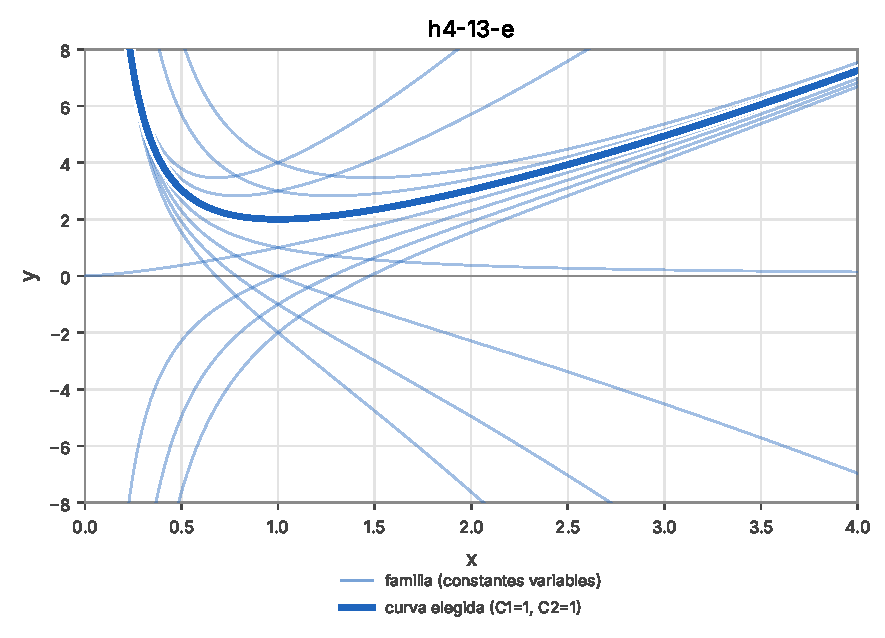
\includegraphics[width=0.8\linewidth]{h4-13-e.pdf}
\end{center}
\item \textbf{(f) $\bm{x^2y''+xy'-16y=0}$:} $s^2 - 16 = 0 \implies s = \pm 4$. $\quad \boxed{y(x) = C_1 x^4 + C_2 x^{-4}}$

\begin{center}
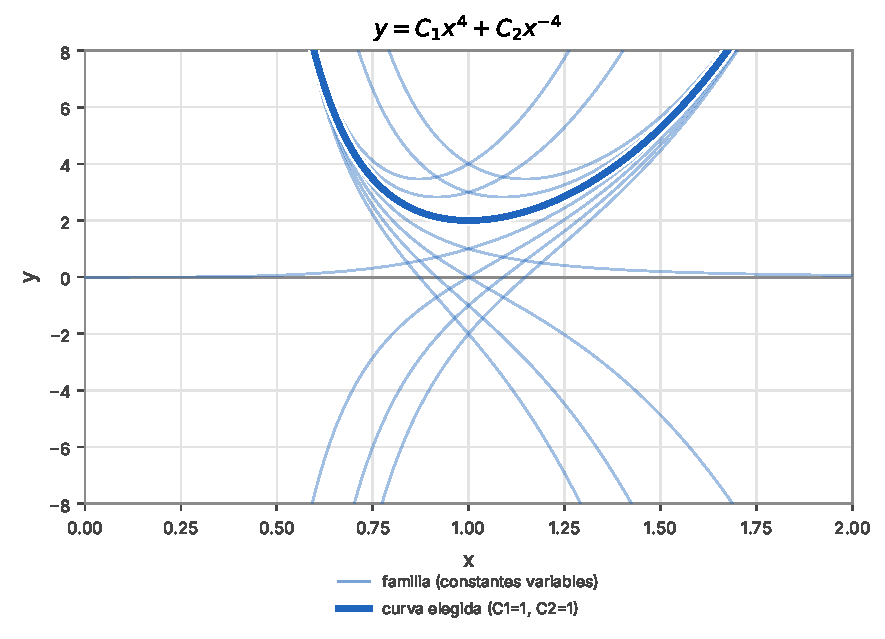
\includegraphics[width=0.8\linewidth]{h4-13-f.pdf}
\end{center}
\end{itemize}

\noindent\textbf{14. En el problema anterior se han transformado ciertas ecuaciones homogéneas con coeficientes variables en ecuaciones con coeficientes constantes cambiando la variable independiente. Considérese la ecuación homogénea general $\bm{y''+P(x)y'+Q(x)y=0}$ y hagamos el cambio de variable independiente de $\bm{x}$ a $\bm{z(x)}$, donde $\bm{z(x)}$ es una función no especificada de $\bm{x}$. Demostrad que la ecuación anterior puede ser transformada de este modo en una ecuación con coeficientes constantes si y sólo si $\bm{(Q'+2PQ)/Q^{3/2}}$ es constante, en cuyo caso $\bm{z=\int\sqrt{Q(x)}\,dx}$ logrará el efecto deseado.} \\
Sea $z=z(x)$ con $z'\neq0$ (invertible). Por la regla de la cadena:
\begin{align*}
\frac{dy}{dx} = z' \frac{dy}{dz}, \qquad \frac{d^2y}{dx^2} = (z')^2 \frac{d^2y}{dz^2} + z'' \frac{dy}{dz}
\end{align*}
Sustituyendo en la EDO y dividiendo entre $(z')^2$:
\begin{align*}
\frac{d^2y}{dz^2} + \underbrace{\frac{z'' + P(x)z'}{(z')^2}}_{p(x)} \frac{dy}{dz} + \underbrace{\frac{Q(x)}{(z')^2}}_{q(x)} y = 0
\end{align*}
La ecuación tiene coeficientes constantes si y sólo si $p(x)$ y $q(x)$ son constantes. Suponemos $Q>0$ en el intervalo considerado (para que $\sqrt{Q}$ y $Q^{3/2}$ sean reales y el cociente esté definido).

\vspace{0.2cm}\noindent\textbf{($\Rightarrow$) Directo.} Supongamos que existe $z(x)$ con $p$ y $q$ constantes y probemos que $\dfrac{Q'+2PQ}{Q^{3/2}}$ es constante. Como $Q>0$ y $(z')^2>0$, $q=Q/(z')^2>0$ y de ahí $(z')^2=Q/q$. Tomando $z'>0$ (si $z'<0$ solo cambia el signo de la constante final): $z'=\sqrt{Q/q}$. Derivando $(z')^2=Q/q$ obtenemos $2z'z''=Q'/q$, es decir $z''=\dfrac{Q'}{2qz'}$. De la definición de $p$:
\begin{align*}
p\,(z')^2 = z''+Pz' \implies p\,(z')^3 = z'z''+P(z')^2 = \frac{Q'}{2q} + \frac{PQ}{q} = \frac{Q'+2PQ}{2q}
\end{align*}
Como $(z')^3 = Q^{3/2}/q^{3/2}$:
\begin{align*}
\frac{Q'+2PQ}{Q^{3/2}} = \frac{2q\,p}{q^{3/2}} = \frac{2p}{\sqrt{q}} = \text{constante} \quad \blacksquare
\end{align*}

\vspace{0.2cm}\noindent\textbf{($\Leftarrow$) Inverso.} Supongamos ahora $\dfrac{Q'+2PQ}{Q^{3/2}}=C$ constante y probemos que $z=\int\sqrt{Q(x)}\,dx$ transforma la ecuación en una de coeficientes constantes. Con $z'=\sqrt{Q}$:
\begin{align*}
q = \frac{Q}{(z')^2} = 1, \qquad z'' = \frac{Q'}{2\sqrt{Q}} \implies p = \frac{\frac{Q'}{2\sqrt{Q}} + P\sqrt{Q}}{Q} = \frac{Q'+2PQ}{2Q^{3/2}} = \frac{C}{2}
\end{align*}
Ambos son constantes y la ecuación queda
\[
\frac{d^2y}{dz^2} + \frac{C}{2}\frac{dy}{dz} + y = 0 \quad \blacksquare
\]

\noindent\textbf{15. Usad el resultado del problema anterior y resolved cuando sea posible:}

\begin{itemize}
\item \textbf{(a) $\bm{xy''+(x^2-1)y'+x^3y=0} \implies y'' + \left(x - \frac{1}{x}\right)y' + x^2 y = 0$:} \\
$P(x) = x - 1/x, \, Q(x) = x^2 \implies \frac{Q'+2PQ}{Q^{3/2}} = \frac{2x + 2(x-1/x)x^2}{x^3} = 2$ (constante). \\
$z = \int x \, dx = \frac{x^2}{2} \implies \frac{d^2y}{dz^2} + \frac{dy}{dz} + y = 0 \implies s = -\frac{1}{2} \pm i\frac{\sqrt{3}}{2}$.
\[
\boxed{y(x) = e^{-x^2/4}\left(C_1 \cos\frac{\sqrt{3}x^2}{4} + C_2 \sin\frac{\sqrt{3}x^2}{4}\right)}
\]


\begin{center}
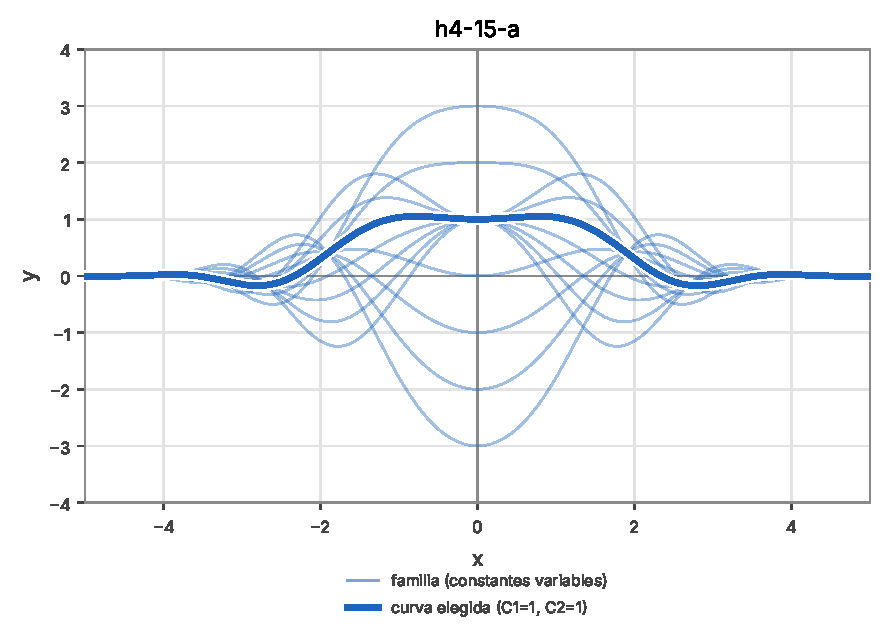
\includegraphics[width=0.8\linewidth]{h4-15-a.pdf}
\end{center}
\item \textbf{(b) $\bm{y''+3xy'+x^2y=0}$:} \\
$P(x) = 3x, \, Q(x) = x^2 \implies \frac{Q'+2PQ}{2Q^{3/2}} = \frac{2x + 6x^3}{2x^3} = 3 + \frac{1}{x^2}$ (no es constante).
\[
\boxed{\text{No es posible transformarla en coeficientes constantes.}}
\]
\end{itemize}


\noindent\textbf{16. Hallad la solución general de las siguientes ecuaciones no homogéneas:}

\begin{itemize}
\item \textbf{(a) $\bm{y''-y'-6y=20e^{-2x}}$:} \\
$y_h = C_1 e^{3x} + C_2 e^{-2x}$. Proponemos $y_p = A x e^{-2x} \implies y_p'' - y_p' - 6y_p = -5A e^{-2x} = 20e^{-2x} \implies A = -4$.
\[
\boxed{y(x) = C_1 e^{3x} + C_2 e^{-2x} - 4x e^{-2x}}
\]


\begin{center}
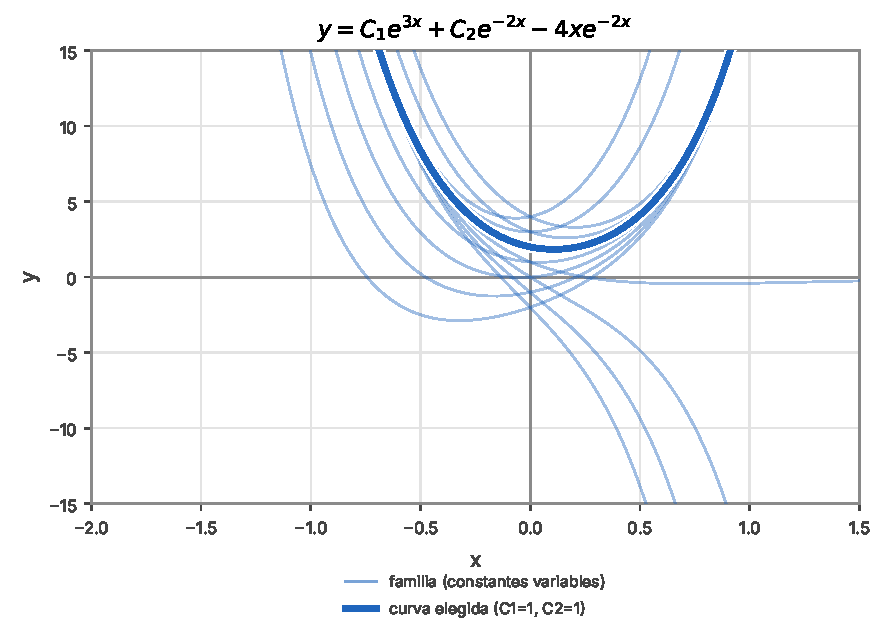
\includegraphics[width=0.8\linewidth]{h4-16-a.pdf}
\end{center}
\item \textbf{(b) $\bm{y''-3y'+2y=14\sin 2x - 18\cos 2x}$:} \\
$y_h = C_1 e^x + C_2 e^{2x}$. Proponemos $y_p = A\cos 2x + B\sin 2x$. Sustituyendo e igualando:
\begin{align*}
(-2A - 6B)\cos 2x + (6A - 2B)\sin 2x = -18\cos 2x + 14\sin 2x \implies A = 3, \quad B = 2
\end{align*}
\[
\boxed{y(x) = C_1 e^x + C_2 e^{2x} + 3\cos 2x + 2\sin 2x}
\]


\begin{center}
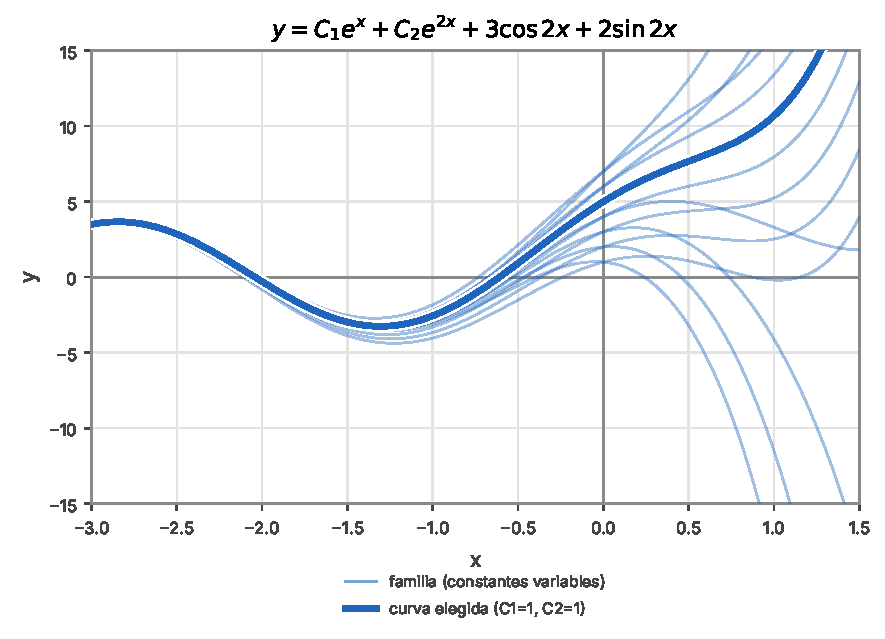
\includegraphics[width=0.8\linewidth]{h4-16-b.pdf}
\end{center}
\item \textbf{(c) $\bm{y''+y=2\cos x}$:} \\
$y_h = C_1 \cos x + C_2 \sin x$. Por doble cero, $y_p = x(A\cos x + B\sin x) \implies y_p'' + y_p = -2A\sin x + 2B\cos x = 2\cos x \implies A = 0, B = 1$.
\[
\boxed{y(x) = C_1 \cos x + C_2 \sin x + x \sin x}
\]


\begin{center}
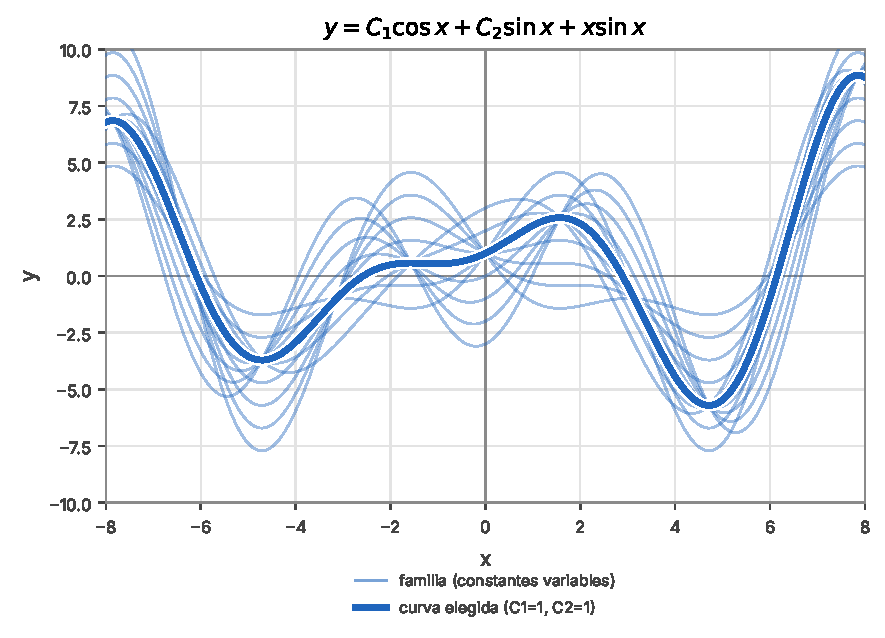
\includegraphics[width=0.8\linewidth]{h4-16-c.pdf}
\end{center}
\item \textbf{(d) $\bm{y''-2y'=12x-10}$:} \\
$y_h = C_1 + C_2 e^{2x}$. Proponemos $y_p = Ax^2 + Bx \implies y_p'' - 2y_p' = -4Ax + (2A - 2B) = 12x - 10 \implies A = -3, B = 2$.
\[
\boxed{y(x) = C_1 + C_2 e^{2x} - 3x^2 + 2x}
\]


\begin{center}
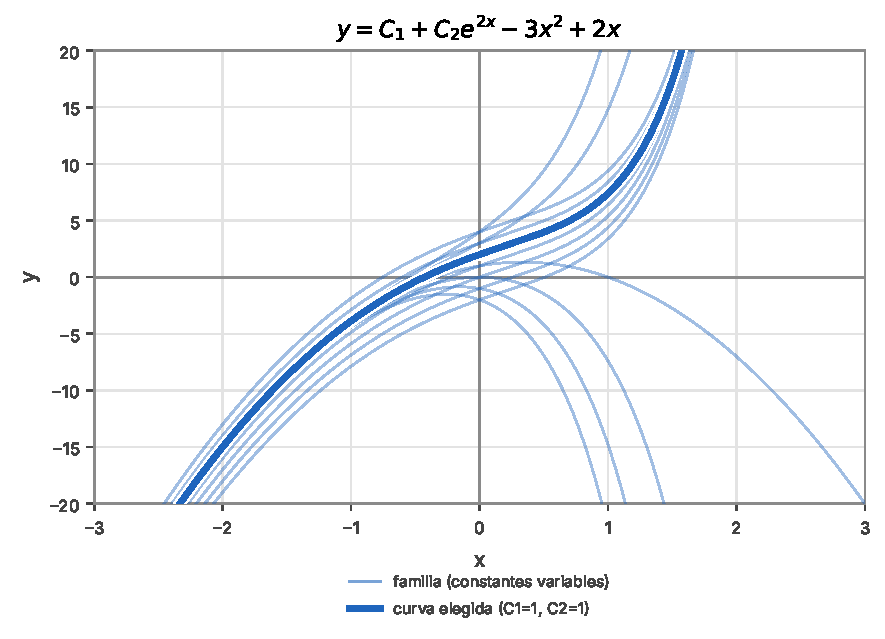
\includegraphics[width=0.8\linewidth]{h4-16-d.pdf}
\end{center}
\item \textbf{(e) $\bm{y''-2y'+y=6e^x}$:} \\
$y_h = (C_1 + C_2 x)e^x$. $y_p = A x^2 e^x \implies y_p'' - 2y_p' + y_p = 2A e^x = 6e^x \implies A = 3$.
\[
\boxed{y(x) = (C_1 + C_2 x + 3x^2)e^x}
\]


\begin{center}
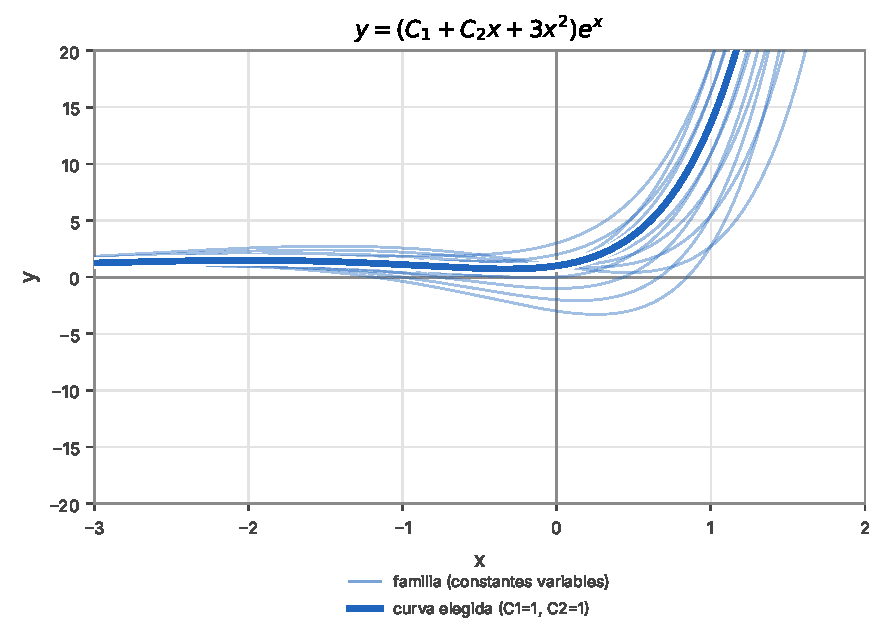
\includegraphics[width=0.8\linewidth]{h4-16-e.pdf}
\end{center}
\item \textbf{(f) $\bm{y''-2y'+2y=e^x \sin x}$:} \\
$y_h = e^x(C_1 \cos x + C_2 \sin x)$. Por doble cero, $y_p = x e^x (A\cos x + B\sin x) \implies A = -1/2, B = 0$.
\[
\boxed{y(x) = e^x(C_1 \cos x + C_2 \sin x) - \frac{1}{2}x e^x \cos x}
\]


\begin{center}
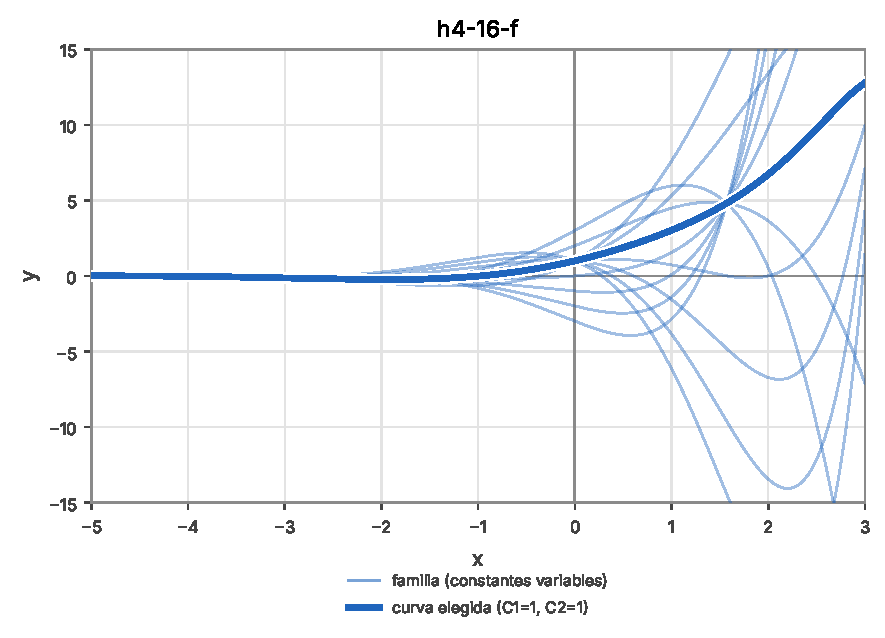
\includegraphics[width=0.8\linewidth]{h4-16-f.pdf}
\end{center}
\item \textbf{(g) $\bm{y''+y'=10x^4+2}$:} \\
$y_h = C_1 + C_2 e^{-x}$. Proponemos (porque la edo no tiene término con y) $y_p = x(Ax^4 + Bx^3 + Cx^2 + Dx + E)   \implies A=2, B=-10, C=40, D=-120, E=242$.
\[
\boxed{y(x) = C_1 + C_2 e^{-x} + 2x^5 - 10x^4 + 40x^3 - 120x^2 + 242x}
\]


\begin{center}
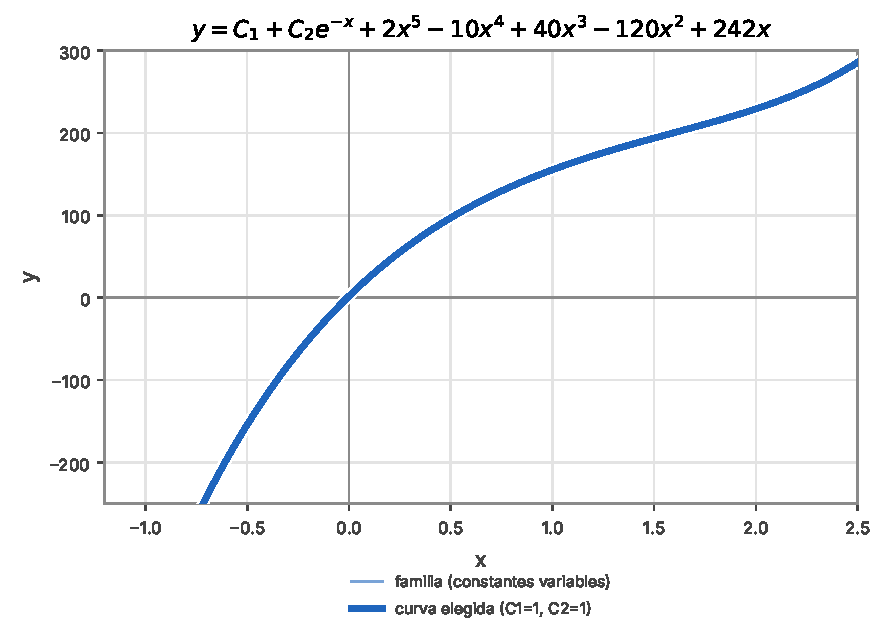
\includegraphics[width=0.8\linewidth]{h4-16-g.pdf}
\end{center}
\item \textbf{(h) $\bm{y''+9y=2\sin 3x + 4\sin x - 26e^{-2x} + 27x^3}$:} \\
$s^2 + 9 = 0 \implies s = \pm 3i$,
\begin{align*}
y_h(x) = C_1 \cos 3x + C_2 \sin 3x
\end{align*}
Dividimos el término no homogéneo en cuatro partes:
\begin{itemize}
\item \textbf{Para $\bm{f_1(x) = 2\sin 3x}$ (Cero de la caracteristica):} proponemos $y_{p1} = x(A\cos 3x + B\sin 3x)$. Sustituyendo: $-6A\sin 3x = 2\sin 3x \implies A = -1/3, B = 0$.
\[
y_{p1}(x) = -\frac{1}{3}x\cos 3x
\]
\item \textbf{Para $\bm{f_2(x) = 4\sin x}$:} proponemos $y_{p2} = C\cos x + D\sin x$. Sustituyendo se llega a $8D\sin x = 4\sin x \implies C = 0, D = 1/2$.
\[
y_{p2}(x) = \frac{1}{2}\sin x
\]
\item \textbf{Para $\bm{f_3(x) = -26e^{-2x}}$:} proponemos $y_{p3} = Ee^{-2x}$. Sustituyendo se obtiene $13Ee^{-2x} = -26e^{-2x} \implies E = -2$.
\[
y_{p3}(x) = -2e^{-2x}
\]
\item \textbf{Para $\bm{f_4(x) = 27x^3}$:} proponemos un polinomio general de tercer grado $y_{p4} = Fx^3 + Gx^2 + Hx + I$. Al sustituir e igualar coeficientes se determina que $F=3, G=0, H=-2, I=0$.
\[
y_{p4}(x) = 3x^3 - 2x
\]
\end{itemize}
Sumando la solución homogénea y todas las soluciones particulares obtenidas:
\[
\boxed{y(x) = C_1 \cos 3x + C_2 \sin 3x - \frac{1}{3}x\cos 3x + \frac{1}{2}\sin x - 2e^{-2x} + 3x^3 - 2x}
\]

\begin{center}
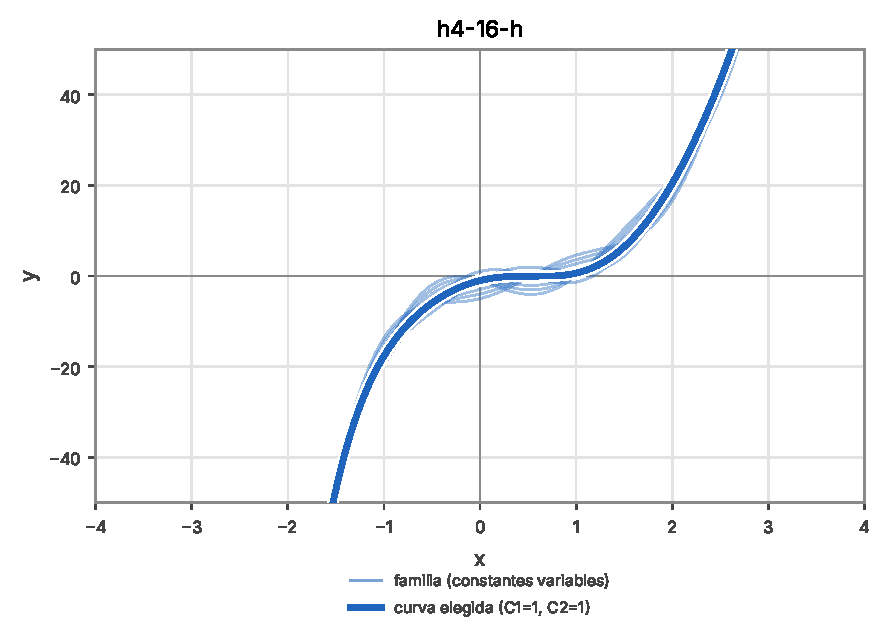
\includegraphics[width=0.8\linewidth]{h4-16-h.pdf}
\end{center}
\end{itemize}


\noindent\textbf{17. Hallad una solución particular por variación de parámetros:} \\
Antes de resolver, se deduce el método visto en clase para la EDO general $y'' + P(x)y' + Q(x)y = f(x)$. variando las constantes:
\begin{align*}
y_p(x) = u_1(x)y_1(x) + u_2(x)y_2(x)
\end{align*}
Derivando e imponiendo la condición $u_1'y_1 + u_2'y_2 = 0$ para evitar derivadas de orden superior en las incógnitas, obtenemos el sistema:
\begin{align*}
\begin{cases} u_1'y_1 + u_2'y_2 = 0 \\ u_1'y_1' + u_2'y_2' = f(x) \end{cases}
\end{align*}
\begin{align*}
\begin{pmatrix} y_1 & y_2 \\ y_1' & y_2' \end{pmatrix} \begin{pmatrix} u_1' \\ u_2' \end{pmatrix} = \begin{pmatrix} 0 \\ f(x) \end{pmatrix}
\end{align*}
Invertimos la matriz de coeficientes (det es el Wronskiano $W = y_1y_2' - y_1'y_2 \neq 0$):
\begin{align*}
\begin{pmatrix} u_1' \\ u_2' \end{pmatrix} = \frac{1}{W} \begin{pmatrix} y_2' & -y_2 \\ -y_1' & y_1 \end{pmatrix} \begin{pmatrix} 0 \\ f(x) \end{pmatrix} = \frac{1}{W} \begin{pmatrix} -y_2 f(x) \\ y_1 f(x) \end{pmatrix}
\end{align*}

\begin{align*}
u_1' = -\frac{y_2 f(x)}{W} \implies u_1(x) = -\int \frac{y_2 f(x)}{W} dx, \qquad u_2' = \frac{y_1 f(x)}{W} \implies u_2(x) = \int \frac{y_1 f(x)}{W} dx
\end{align*}

\begin{itemize}
\item \textbf{(a) $\bm{y''+4y=\tan 2x}$:} \\
$y''+4y=0 \implies s^2+4=0 \implies s=\pm 2i$. 
\begin{align*}
y_1(x) &= \cos(2x) \\
y_2(x) &= \sin(2x)
\end{align*}
\begin{align*}
W = \begin{vmatrix} \cos(2x) & \sin(2x) \\ -2\sin(2x) & 2\cos(2x) \end{vmatrix} = 2\cos^2(2x) + 2\sin^2(2x) = 2
\end{align*}
Aplicamos las fórmulas de variación de parámetros con $f(x) = \tan(2x)$:
\begin{align*}
u_1'(x) &= -\frac{y_2(x)f(x)}{W} = -\frac{\sin(2x)\tan(2x)}{2} = -\frac{1}{2}\frac{\sin^2(2x)}{\cos(2x)} = -\frac{1}{2}\frac{1-\cos^2(2x)}{\cos(2x)} = -\frac{1}{2}\big(\sec(2x) - \cos(2x)\big) \\
u_1(x) &= -\frac{1}{2}\int \big(\sec(2x) - \cos(2x)\big)dx = -\frac{1}{4}\ln|\sec(2x) + \tan(2x)| + \frac{1}{4}\sin(2x)
\end{align*}
\begin{align*}
u_2'(x) &= \frac{y_1(x)f(x)}{W} = \frac{\cos(2x)\tan(2x)}{2} = \frac{\sin(2x)}{2} \\
u_2(x) &= \frac{1}{2}\int \sin(2x)dx = -\frac{1}{4}\cos(2x)
\end{align*}
Sustituyendo en la solución particular $y_p(x) = u_1(x)y_1(x) + u_2(x)y_2(x)$:
\begin{align*}
y_p(x) &= \left( -\frac{1}{4}\ln|\sec(2x) + \tan(2x)| + \frac{1}{4}\sin(2x) \right)\cos(2x) + \left( -\frac{1}{4}\cos(2x) \right)\sin(2x) \\
y_p(x) &= -\frac{1}{4}\cos(2x)\ln|\sec(2x) + \tan(2x)| + \frac{1}{4}\sin(2x)\cos(2x) - \frac{1}{4}\sin(2x)\cos(2x)
\end{align*}
\[
\boxed{y_p(x) = -\frac{1}{4}\cos(2x)\ln|\sec(2x) + \tan(2x)|}
\]

\begin{center}
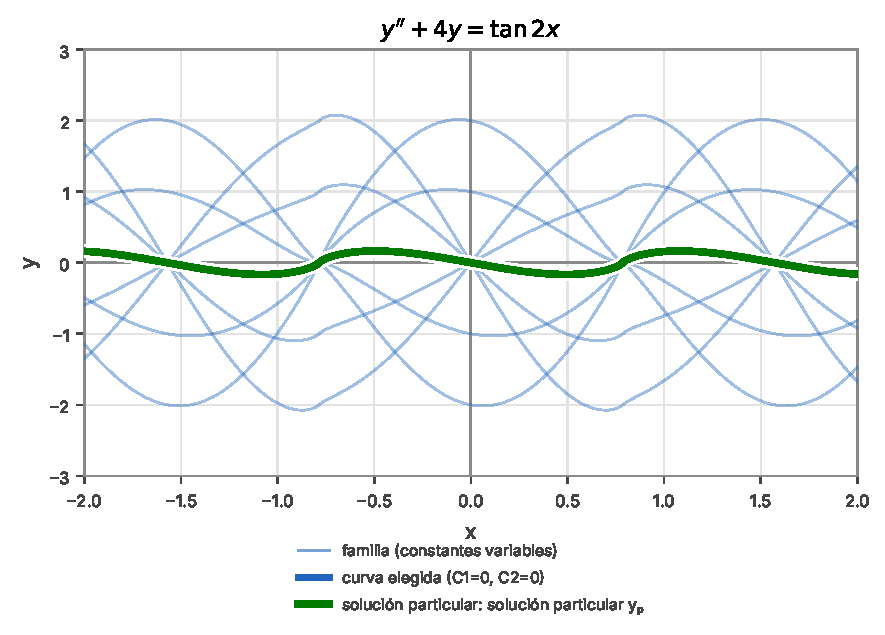
\includegraphics[width=0.8\linewidth]{h4-17-a.pdf}
\end{center}
\item \textbf{(b) $\bm{y''+2y'+y=e^{-x}\ln x}$:} \\
$y_1 = e^{-x}, y_2 = x e^{-x}, W = e^{-2x}$. $u_1' = -x\ln x \implies u_1 = -\frac{x^2}{2}\ln x + \frac{x^2}{4}$. $u_2' = \ln x \implies u_2 = x\ln x - x$.
\[
\boxed{y_p(x) = \frac{1}{2}x^2 e^{-x}\ln x - \frac{3}{4}x^2 e^{-x}}
\]

\begin{center}
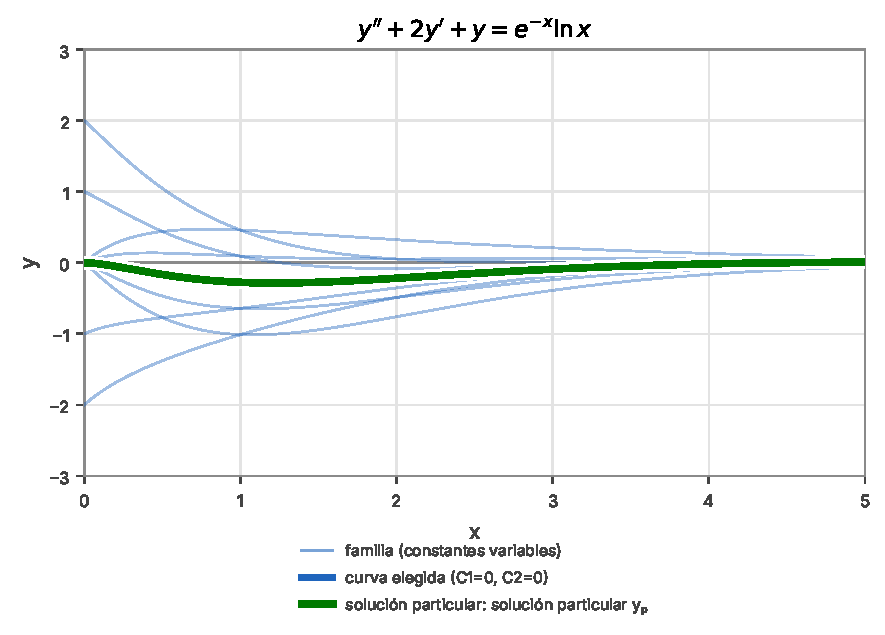
\includegraphics[width=0.8\linewidth]{h4-17-b.pdf}
\end{center}
\item \textbf{(c) $\bm{y''-2y'-3y=64xe^{-x}}$:} \\
$y''-2y'-3y=0 \implies s^2-2s-3=0 \implies s_1=3, s_2=-1$. \\
Como el término no homogéneo es $64xe^{-x}$ y $s=-1$ es raíz, tenemos un caso similar a cuando es doble. Proponemos la solución particular multiplicada por $x$:
\begin{align*}
y_p(x) &= x(Ax+B)e^{-x} = (Ax^2+Bx)e^{-x} \\
y_p'(x) &= (-Ax^2 + (2A-B)x + B)e^{-x} \\
y_p''(x) &= (Ax^2 + (-4A+B)x + 2A-2B)e^{-x}
\end{align*}
Sustituimos en la EDO original y agrupamos por potencias de $x$:
\begin{align*}
y_p'' - 2y_p' - 3y_p &= e^{-x}\big[ (A+2A-3A)x^2 + (-4A+B-4A+2B-3B)x + (2A-2B-2B) \big] \\
&= e^{-x}\big[ 0x^2 - 8Ax + (2A-4B) \big] = 64xe^{-x}
\end{align*}
Igualando coeficientes obtenemos el sistema:
\begin{align*}
\begin{cases} -8A = 64 \implies A = -8 \\ 2A - 4B = 0 \implies 2(-8) - 4B = 0 \implies B = -4 \end{cases}
\end{align*}
\[
\boxed{y_p(x) = (-8x^2 - 4x)e^{-x}}
\]


\begin{center}
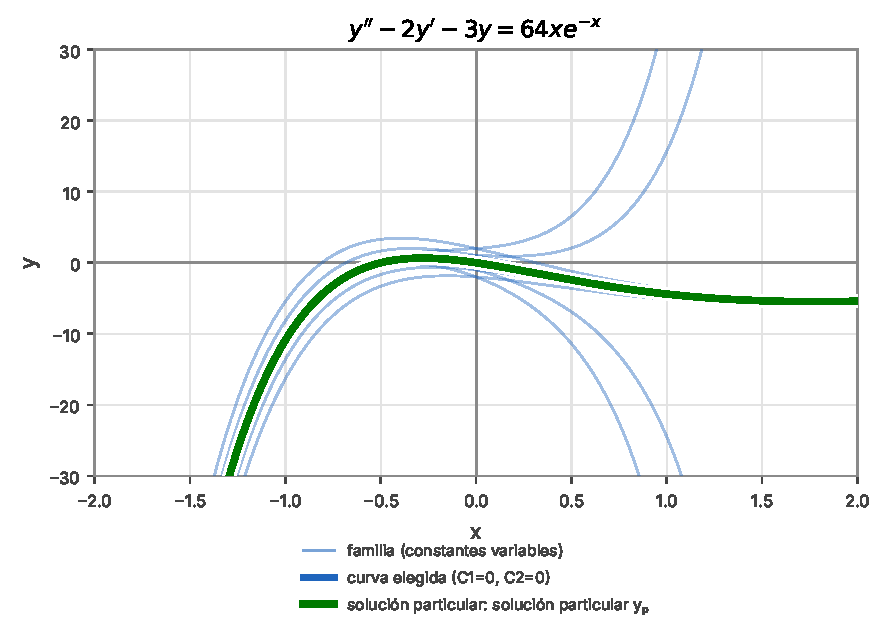
\includegraphics[width=0.8\linewidth]{h4-17-c.pdf}
\end{center}
\item \textbf{(d) $\bm{y''+2y'+5y=e^{-x}\sec 2x}$:} \\
Proponemos el cambio de variable dependiente $y(x) = z(x)e^{-x}$. Basicamente proque eso nos permite eliminar $e^{-x}$ que se convervara en las derivadas. Derivamos usando la regla del producto:
\begin{align*}
y' &= (z' - z)e^{-x} \\
y'' &= (z'' - 2z' + z)e^{-x}
\end{align*}
Sustituyendo en la EDO original y factorizando la exponencial:
\begin{align*}
(z'' - 2z' + z)e^{-x} + 2(z' - z)e^{-x} + 5z e^{-x} &= e^{-x}\sec 2x \\
e^{-x}(z'' - 2z' + z + 2z' - 2z + 5z) &= e^{-x}\sec 2x \implies z'' + 4z = \sec 2x
\end{align*}
Resolvemos esta nueva EDO por el método de variación. La homogénea es $z''+4z=0 \implies z_1 = \cos 2x, \, z_2 = \sin 2x$, con Wronskiano $W = 2$.
\begin{align*}
u_1' &= -\frac{\sin(2x)\sec(2x)}{2} = -\frac{1}{2}\tan(2x) \implies u_1 = -\frac{1}{2}\int \frac{\sin 2x}{\cos 2x}dx = \frac{1}{4}\ln|\cos 2x| \\
u_2' &= \frac{\cos(2x)\sec(2x)}{2} = \frac{1}{2} \implies u_2 = \int \frac{1}{2}dx = \frac{x}{2}
\end{align*}
La solución particular para la variable transformada $z$ es: 
\begin{align*}
z_p(x) = u_1 z_1 + u_2 z_2 = \frac{1}{4}\cos(2x)\ln|\cos 2x| + \frac{x}{2}\sin(2x)
\end{align*}
Deshaciendo el cambio de variable ($y_p = z_p e^{-x}$):
\[
\boxed{y_p(x) = e^{-x}\left(\frac{1}{4}\cos(2x)\ln|\cos 2x| + \frac{x}{2}\sin(2x)\right)}
\]

\begin{center}
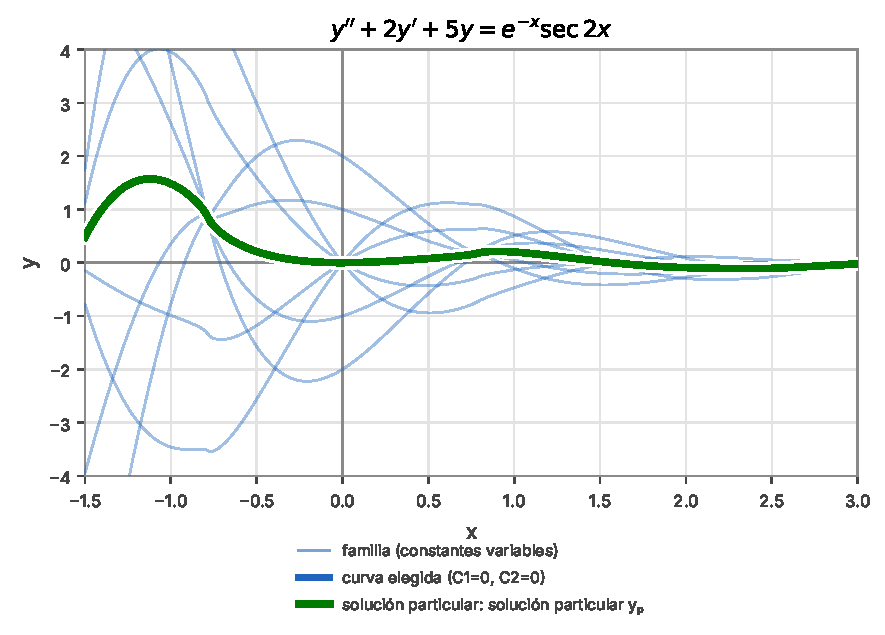
\includegraphics[width=0.8\linewidth]{h4-17-d.pdf}
\end{center}
\item \textbf{(e) $\bm{2y''+3y'+y=e^{-3x}}$:}
\[
\boxed{y_p(x) = \frac{1}{10}e^{-3x}}
\]


\begin{center}
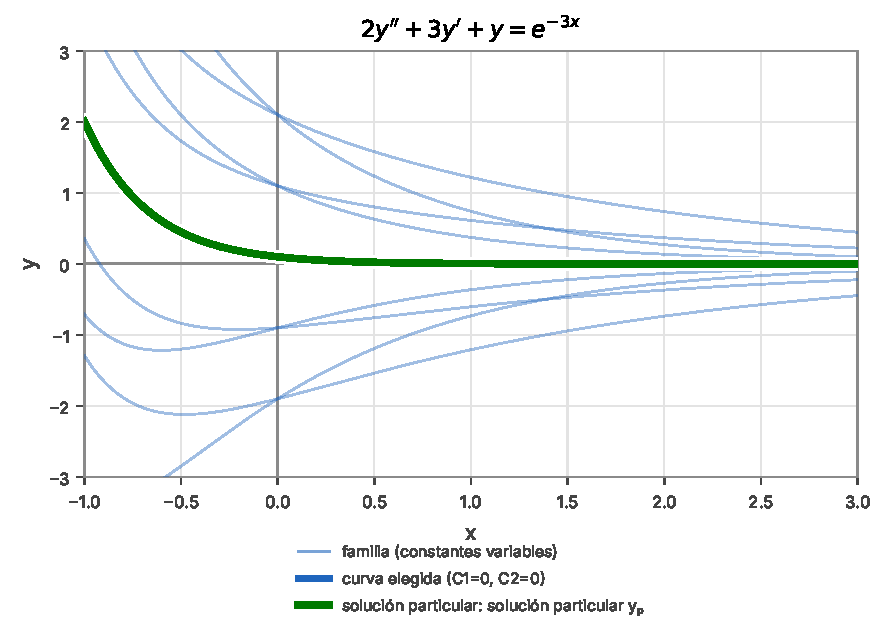
\includegraphics[width=0.8\linewidth]{h4-17-e.pdf}
\end{center}
\item \textbf{(f) $\bm{y''-3y'+2y=\frac{1}{1+e^{-x}}}$:} \\
$y_1 = e^x, y_2 = e^{2x}, W = e^{3x}$. Integrando las expresiones de $u_1'$ y $u_2'$:
\[
\boxed{y_p(x) = (e^x + e^{2x})\ln(1+e^{-x}) - e^x}
\]

\begin{center}
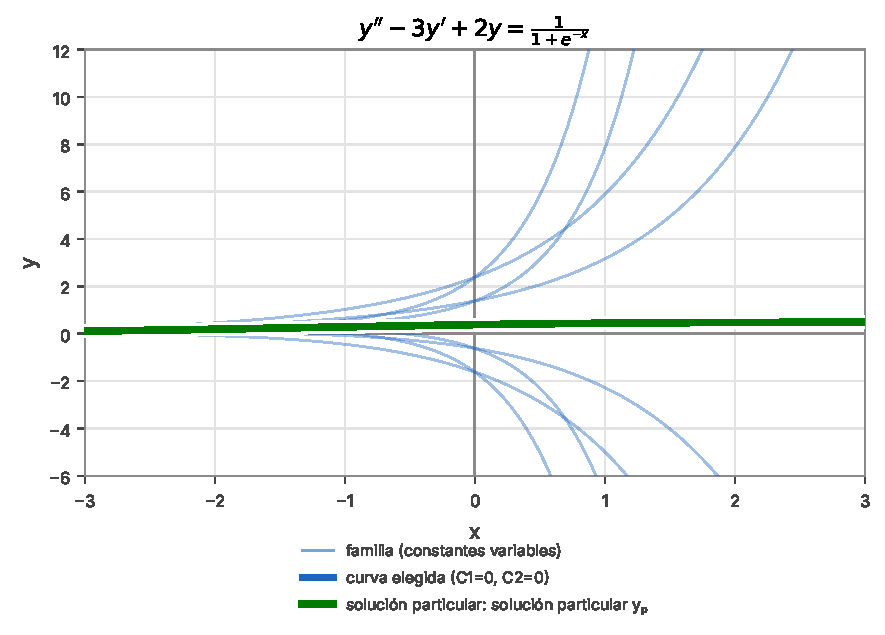
\includegraphics[width=0.8\linewidth]{h4-17-f.pdf}
\end{center}
\end{itemize}

\noindent\textbf{19. Demostrad que el método de variación de los parámetros aplicado a $\bm{y''+y=f(x)}$ conduce a $\bm{y_p(x)=\int_0^x f(t)\sin(x-t)dt}$. Hallad la fórmula para $\bm{y''+k^2y=f(x)}$ con $\bm{k>0}$.}

\noindent Para $y''+y=f(x)$, las soluciones homogéneas son $y_1(x) = \cos x$ e $y_2(x) = \sin x$ con $W=1$.
\begin{align*}
u_1(x) = -\int_0^x f(t)\sin t \, dt, \qquad u_2(x) = \int_0^x f(t)\cos t \, dt
\end{align*}
\begin{align*}
y_p(x) &= u_1(x)\cos x + u_2(x)\sin x = \int_0^x f(t) \big[\sin x \cos t - \cos x \sin t\big] dt = \int_0^x f(t)\sin(x-t) dt \quad \blacksquare
\end{align*}
Para $y''+k^2 y = f(x)$, $y_1(x) = \cos(kx)$ e $y_2(x) = \sin(kx)$ con $W = k$:
\begin{align*}
u_1(x) = -\frac{1}{k}\int_0^x f(t)\sin(kt) \, dt, \qquad u_2(x) = \frac{1}{k}\int_0^x f(t)\cos(kt) \, dt
\end{align*}
\[
\boxed{y_p(x) = \frac{1}{k}\int_0^x f(t)\sin(k(x-t)) \, dt}
\]

\noindent\textbf{18. Hallad una solución particular de $\bm{y''+y=f(x)}$ ($\bm{y_1=\cos x, y_2=\sin x, W=1}$):}

\begin{itemize}
\item \textbf{(a) $\bm{f(x)=\sec x}$:} $\quad \boxed{y_p(x) = \cos x \ln|\cos x| + x \sin x}$

\begin{center}
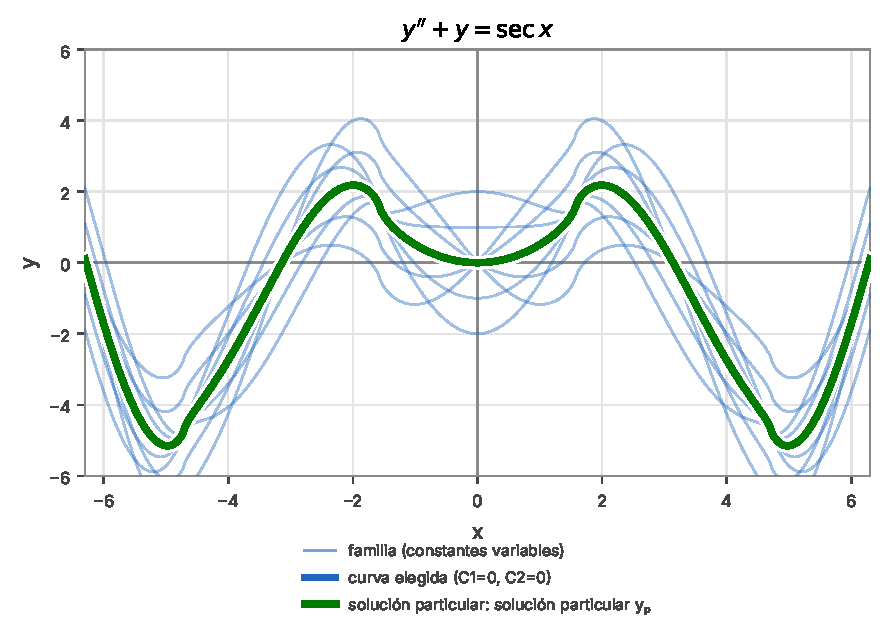
\includegraphics[width=0.8\linewidth]{h4-18-a.pdf}
\end{center}
\item \textbf{(b) $\bm{f(x)=\cot^2 x}$:} $\quad \boxed{y_p(x) = \cos x \ln|\csc x + \cot x| - 2}$

\begin{center}
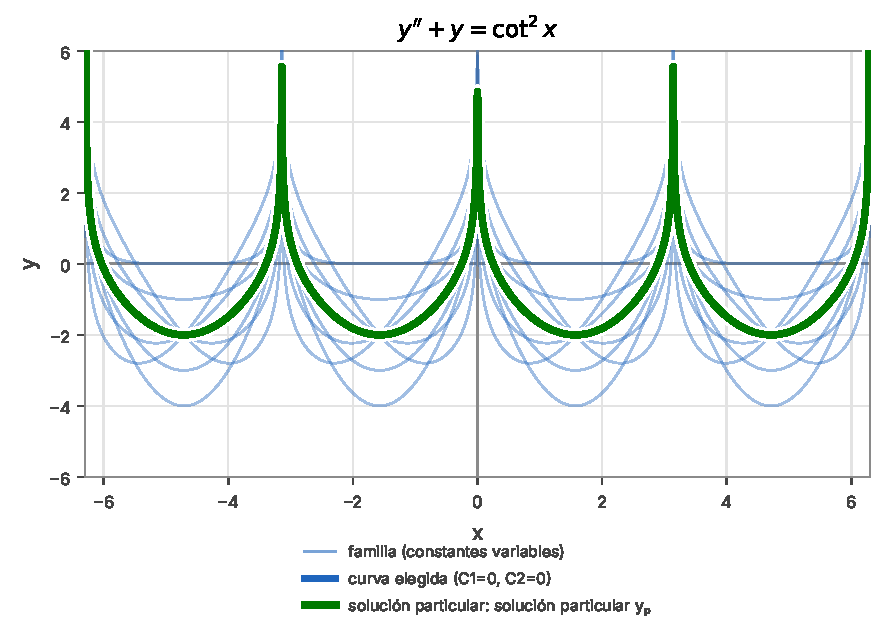
\includegraphics[width=0.8\linewidth]{h4-18-b.pdf}
\end{center}
\item \textbf{(c) $\bm{f(x)=\cot 2x}$:} $\quad \boxed{y_p(x) = \frac{1}{2}\cos x \ln|\sec x + \tan x| - \frac{1}{2}\sin x \ln|\csc x + \cot x|}$

\begin{center}
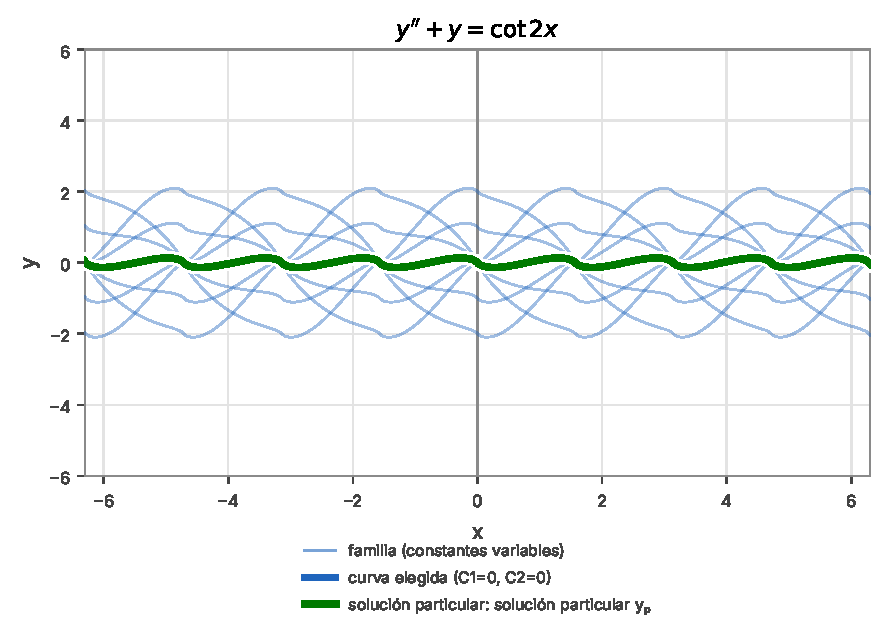
\includegraphics[width=0.8\linewidth]{h4-18-c.pdf}
\end{center}
\item \textbf{(d) $\bm{f(x)=x\cos x}$:} $\quad \boxed{y_p(x) = \frac{x^2}{4}\sin x + \frac{x}{4}\cos x}$

\begin{center}
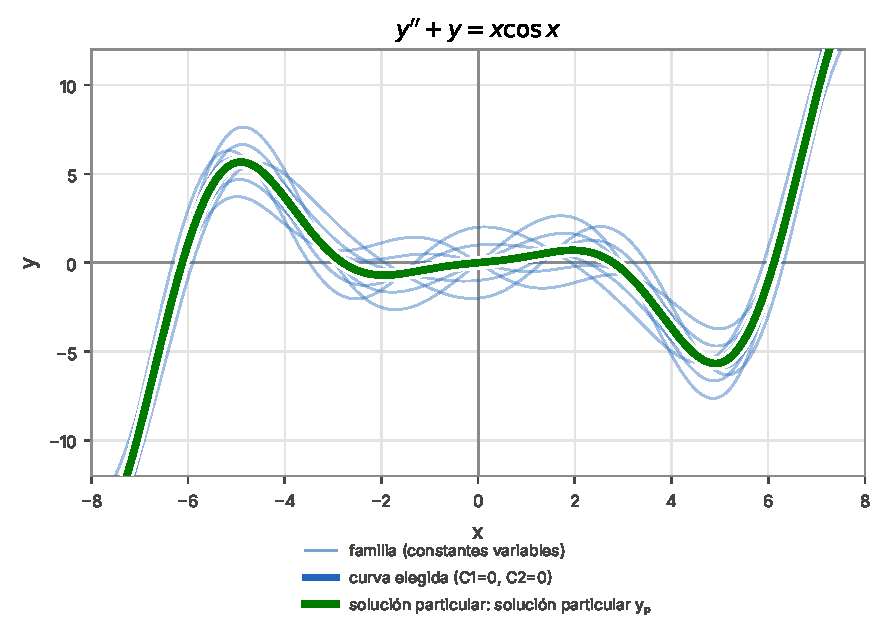
\includegraphics[width=0.8\linewidth]{h4-18-d.pdf}
\end{center}
\item \textbf{(e) $\bm{f(x)=\tan x}$:} $\quad \boxed{y_p(x) = -\cos x \ln|\sec x + \tan x|}$

\begin{center}
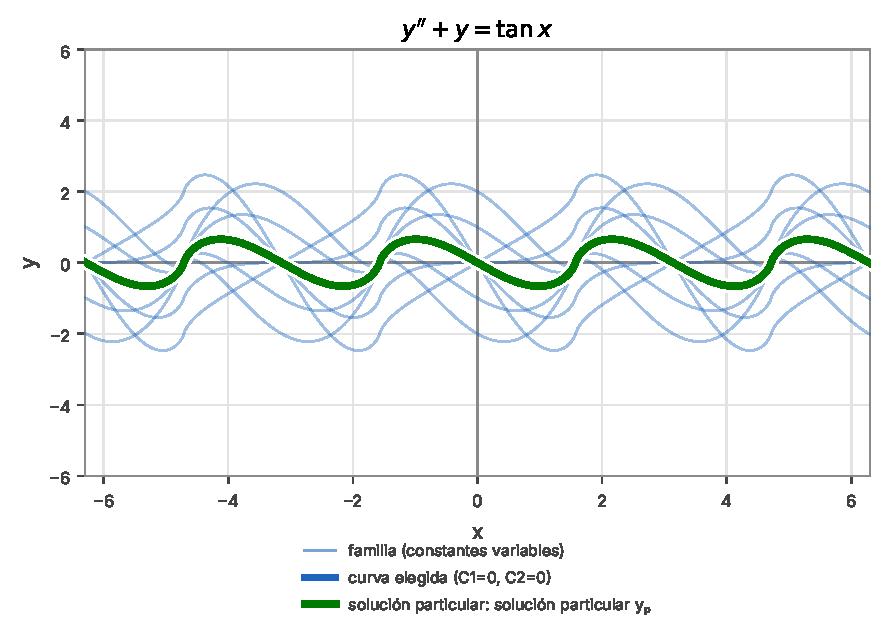
\includegraphics[width=0.8\linewidth]{h4-18-e.pdf}
\end{center}
\item \textbf{(f) $\bm{f(x)=\sec x\tan x}$:} $\quad \boxed{y_p(x) = x\cos x + \sin x \ln|\sec x|}$

\begin{center}
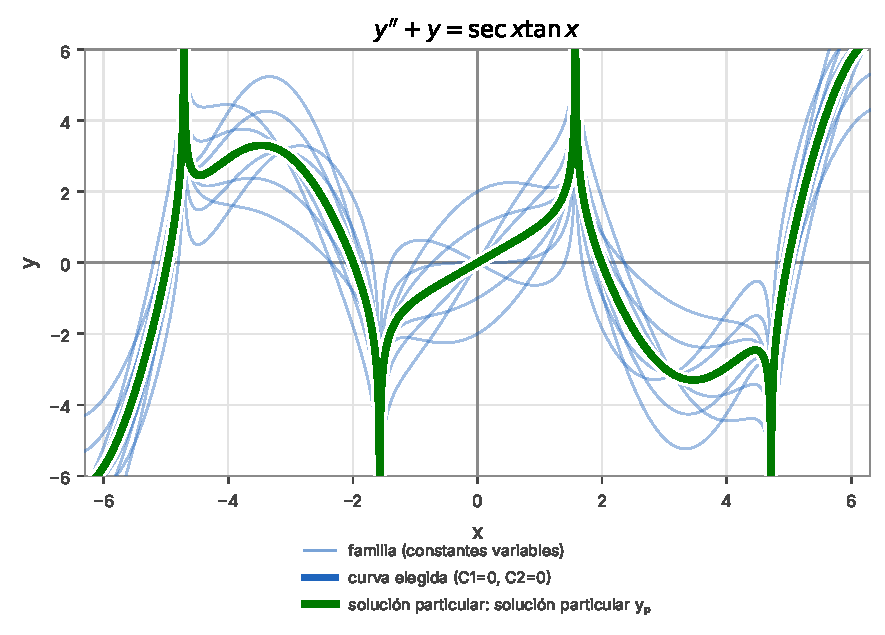
\includegraphics[width=0.8\linewidth]{h4-18-f.pdf}
\end{center}
\item \textbf{(g) $\bm{f(x)=\sec x\csc x}$:} $\quad \boxed{y_p(x) = -\cos x \ln|\sec x + \tan x| - \sin x \ln|\csc x + \cot x|}$

\begin{center}
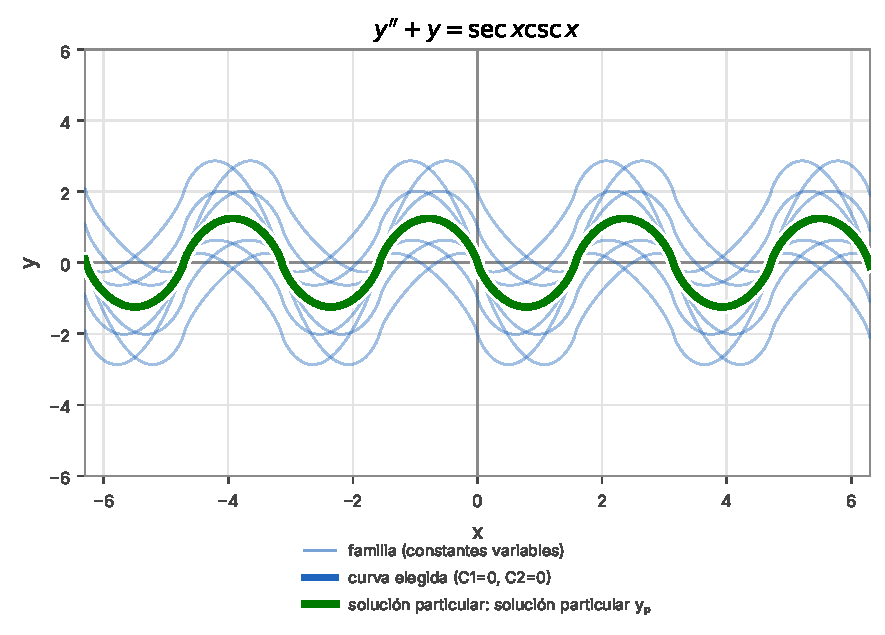
\includegraphics[width=0.8\linewidth]{h4-18-g.pdf}
\end{center}
\end{itemize}

\end{document}
